% !TEX root = ../thesis_main.tex
%
%
%
%%%% --- * --- %%%%	
\clearpage
\chapter{Calibrations and Data Selection}
\label{calibrations_chapter}
\label{dataselection_chapter}
%\note{An almost-direct quote from John follows as the intro statement for Ch.~\ref{calibrations_chapter}.}
In a precision measurement, the bulk of the research is in determining the systematic uncertainties through self-consistent analysis and simulation.  Each detector in this experiment is critical and has independent calibrations and cuts, which are described in detail in this chapter.  Because this analysis was not blinded, there is an increased importance that the choice of cuts should be clearly justified.  The main goal of blinding was nevertheless achieved --- to make sure all analysis is done completely with full redundancy of checks wherever possible --- so the discipline entailed must be described in full detail.
 
%%%Analysis is critical to a precision measurement, as most of the research is in determining systematic uncertainties by self-consistent analysis and simulations.  Each detector in this experiment is critical and has independent calibrations and cuts. 
%%
%%A full explanation is here (and in the following two chapters) justifying choice of the deterministic cuts,
%%because in the analysis in this thesis the data was not blinded.
%%
%%The main goal of blinding was nevertheless achieved-- to make sure all analysis is done
%%completely with full redundancy of checks wherever possible-- so the discipline entailed must
%%be described in full detail.
%%Here there are details of detectors:
%%eMCP
%%rMCP
%%beta DSSD
%%scintillator.

\section{An Overview of Available Data}
\label{sec:data_overview}
%\note{This section must be consolidated and de-Frankenstein-ed.}
%\note{Polarization measurement was conducted on a different set of data, collected in between the measurements used for $A_{\mathrm{\beta}}$ and $b_{\mathrm{Fierz}}$, and at a higher electric field, because we were unable to run both our MCP detectors simultaneously.  }
Although the detection chamber was designed to feature two MCP detectors on opposing sides of an applied electric field intended for simultaneous use (see Section~\ref{section:mcps}), in practice the two detectors produced quite a bit of feedback when operated at the same time.  In order to salvage usable data from the beamtime, it was necessary to run only one detector at a time, but switched which detector was in use every few hours, collecting approximately the same amount of data with each detector (see Tables~\ref{table:runlist_electrons} and~\ref{table:runlist_recoils}).  Thus, the runs are sorted into `electron' and `recoil' runs, depending on what the detector in use was intended to detect.  The data is further split up into several runsets based on when certain settings were adjusted, and the individual runsets have been treated separately for nearly all parts of the analysis.  

% !TEX root = ../thesis_main.tex


\begin{table}[h!!!!tb]
	\begin{center}
	\begin{tabular}{ c || p{1.2cm} | r | l | p{5.8cm} | }
		\multicolumn{4}{l}{Electron Runs} %& \multicolumn{1}{l}{Electron Runs} 
		\\
		\cline{1-3}
		\multicolumn{5}{c}{ }
		\\
			\multicolumn{1}{  c  }{ } & 
				\multicolumn{1}{  c  } { \!\!OP Delay\!\! } &  \multicolumn{1}{ c }{ \!\!Events\!\! }  
				& \multicolumn{1}{ c }{ \!\!Electric Field\!\! } & \multicolumn{1}{ c }{ Runs } 
				\\
			\cline{2-5}
			\multirow{1}{*}{Runset A}	& $300\,\mu s$
										& 0
										& \,\,\,$66.67$ V/cm
										& 314, 362, 363, 383-386, 393. %, 420.
										\\
			\cline{2-5}
			\multirow{1}{*}{Runset B}	& $300\,\mu s$
										& 173,640
										& $150.0$\,\, V/cm
										& 428-437, 440-445.
										\\
			\cline{2-5}
			\multirow{1}{*}{Runset C}	& $700\,\mu s$
										& 18,129
										& $150.0$\,\, V/cm
										& 476, 477.
										\\
			\cline{2-5}
			\multirow{1}{*}{Runset D}	& $400\,\mu s$
										& 207,596
										& $150.0$\,\, V/cm
										& 478-489, 502-505, 510, 513.
										\\
			\cline{2-5}
	\end{tabular}
	\end{center}
	\note{A list of 2014 online runs with potentially usable data.  Runset A was discarded completely due to problems with hardware threshold settings.  There was a QDC module failure before Run 450, so it and all subsequent runs were performed using a different module, and as a result the scintillator calibrations changed slightly at this time.  Anyway, the point of this thing is to show which electron runs and recoil runs go together, for the purposes of evaluating polarization and cloud attributes.}
	\note{Ben doesn't seem to include Runs 436 and 437 in *any* set of good runs.  Is it an oversight?  I think they're perfectly legit electron runs.  They're fairly long runs...}
	\caption[List of Electron Runs]{A list of electron runs and associated parameters.  The ``Events'' column includes only the number of events that passed all cuts.}
%	\note{This table might eventually go away.  Mostly I just want a record of the total `good' counts.  In total, $N=399,365$.}
	\label{table:runlist_electrons}
\end{table}


% !TEX root = ../thesis_main.tex


\begin{table}[h!tb]
	\begin{center}
	\begin{tabular}{ c || r | l | p{7.8cm} | }
		\multicolumn{3}{l}{Recoil Runs}
		\\
		\cline{1-3}
		\multicolumn{4}{c}{ }
		\\
			\multicolumn{1}{  c  }{ } & 
				\multicolumn{1}{  c  } { \!\!OP Delay\!\! } 
				& \multicolumn{1}{ c }{ \!\!Electric Field\!\! } & \multicolumn{1}{ c }{ Runs } 
				\\
			\cline{2-4}
			\multirow{1}{*}{Runset RA}	& $300\,\mu s$
										& 395.0 V/cm
										& 303, 308-313, 318, 326, 327, 328, 340, 342, 343, 
										376, 377, 378, 394, 395, 396, 398-402.
										\\
			\cline{2-4}
			\multirow{1}{*}{Runset RB}	& $300\,\mu s$
										& 535.0 V/cm
										& 409-419, 421-426, 446, 447, 449.
										\\
			\cline{2-4}
			\multirow{1}{*}{Runset RC}	& $700\,\mu s$
										& 395.0 V/cm
										& 450, 454, 455.
										\\
			\cline{2-4}
			\multirow{1}{*}{Runset RD}	& $700\,\mu s$
										& 415.0 V/cm
										& 460-466, 473, 474.
										\\
			\cline{2-4}
			\multirow{1}{*}{Runset RE}	& $400\,\mu s$
										& 415.0 V/cm
										& 491, 497, 498, 499, 509. 
										\\
			\cline{2-4}
	\end{tabular}
	\end{center}
%	\note{This table might eventually go away.  Mostly I just want a record of the total `good' counts.  In total, $N=399,365$.}
	\note{Ben includes 448 as a `good' recoil run.  But I don't.  Why?  Also 451, 451, 453.  ...Also 467,468,469,470,471,472.  Also-also, 492, 493, 494, 495, 496.}
	\caption[List of Recoil Runs]{A list of 2014 online recoil runs and associated parameters.  A count of good events that pass all cuts is not included because different cuts must be used for polarization and trap position data.}
	\label{table:runlist_recoils}
%	\note{I really need to merge the two tables.  :(  ...also, add a new table to show which things should be used with which other things.}
\end{table}



While the beta asymmetry and Fierz interference are best evaluated using the electron runs, the polarization (a dominant uncertainty in the beta asymmetry measurement) and cloud position are best evaluated with recoil runs.  The polarization measurement is the subject of a recent publication (see~\cite{ben_OP}), and the evaluation of cloud position is discussed in Section~\ref{sec:cloud_calibration}.  
%Because the recoil and electron runs are completely separate, there is no danger of statistical double-counting within the polarization and position measurements.  
The recoil runs may also be analyzed in the future as part of a search for right-handed Weak interactions (described further in Chapter~\ref{section_rslow}).

In considering Tables~\ref{table:runlist_electrons} and~\ref{table:runlist_recoils}, we note that Runsets EA and RA were neglected completely during analysis after it was determined that one scintillator had an improperly set hardware threshold such that lower energy betas weren't being detected at all.  Additionally, there was a QDC module failure before Run 450, resulting in an abrupt change in calibration for the two scintillators.  The electric field is larger during recoil runs in an attempt to maximize the fraction of nuclear recoils collected, as well as the separation in TOF between different charge states.  For electron runs, although not all SOEs were collected, the lower electric fields were preferred in order to decrease background events and the sparking incidents.   Although the final analysis uses only the eMCP runs directly, the result could not have been obtained with the same degree of precision had the rMCP data not been present.  

%Runset EA was discarded completely due to problems with hardware threshold settings.  There was a QDC module failure before Run 450, so it and all subsequent runs were performed using a different module, and as a result the scintillator calibrations changed slightly at this time.

%, and each of these runsets contains both electron and recoil runs.  
%These runsets were then treated separately for nearly all parts of the analysis.  

%Runsets A were not used for analysis because it
%In particular, Data Set A was neglected completely during analysis after it was determined that one scintillator had an improperly set hardware threshold such that lower energy betas weren't being detected at all.  Additionally, there was a QDC module failure between Runsets B and C, resulting in an abrupt change in calibration for the two scintillators. 
 
%\note{`The observant reader may find it curious that the listed runsets start at ``B'' and continue alphabetically.  There was initially a ``Runset A'' collected as well, however it was determined later that this data could not be salvaged for use in the final analysis because one of the scinitillators had its hardware threshold set above the compton peak, and without that reference point an accurate calibration could not be performed.'}

%\note{Also, the background was too noisy in Set A I think.  Also, pretty sure there isn't really that much data in Set A at all.  Also-also, Set A has E=66.7, so can't use it for more stats on the other backgrounds. ... Maybe I should just look up what the deal even was with Set A, since I don't really remember.} 

%\note{What did I change between Runsets B and C?  Between Runsets C and D?  ...OP time, yes, but also and one point a PMT(?) (eta:  it was a QDC) blew out and we replaced it, so then the scintillator calibration was a bit different afterward.  Anyway, I should maybe just make a goddamn table.  Table goes here.}
%

%%%%%%%%%\note{imported chunk:
%%%%%%%%%\\
%%%%%%%%%As described in Chapter~\ref{section:mcps}, the science chamber features a series of electrostatic hoops to maintain an electric field to direct positively and negatively charged particles into MCP detectors on opposing sides of the chamber, but it was only possible to operate one MCP detector at a time, so it was necessary to alternate which detector was in use several times between runs so as to be able to collect both types of data.  Although the final analysis uses only the eMCP runs directly, the result could not have been obtained with the same degree of precision had the rMCP data not been present.  
%%%%%%%%%}


%\clearpage
%\afterpage{\clearpage}
%\FloatBarrier
\section{Preliminary Data Selection with the rMCP}
\label{sec:rmcp_cuts}
As described in Chapter~\ref{photoions}, the primary function of the rMCP within the context of this experiment is as a probe of the atom cloud, and it provided a critical check of the cloud's position, size, and polarization state over the course of the beamtime.  The process of cleaning, calibrating, and analyzing this data is described here.  

The two delay lines located just behind the rMCP provide information about hit position.  The principle behind a delay line's operation is relatively straightforward.  The delay line itself is made from a thin wire wound into a flattened coil that covers the area of the microchannel plate.  The second delay line is oriented perpendicular to the first and immediately behind it, but also covers the full area of the microchannel plate.  When a charged particle is incident on the stack of microchannel plates, an electron shower is initiated.  The shower gains strength as it propagates through the MCPs' microchannels, and emerges on the back side of the stack after having been greatly amplified.  

After emerging from the back of the MCP stack, the electron shower is then incident on a delay line, generating an electrical pulse that propagates from the hit point towards both ends of the wire.  Although the wire is conductive, the propagation speed is finite, and this fact is key to extracting the hit position.  The time of arrival for the electrical pulse is recorded at each end of the delay line wire, and it is the difference between the two times that tells where along the wire the original hit occurred.  In general, a single delay line is only precise enough to determine the hit position as projected along the direction perpendicular to its coil's wires.
%and the initial hit position is determined in one dimension by comparing the difference in pulse arrival times at each end of the wire. 
~\aside{how precise is the rMCP supposed to do?  in practice, it wasn't nearly that good.} 
The electron shower continues past the first delay line to hit the delay line immediately behind, which again creates an electrical pulse that propagates towards the ends of that wire, and a similar procedure can be used to evaluate the hit position in the perpendicular direction.  Therefore, for an event~\aside{It's not really *every* event...} in which the rMCP is hit and an electron shower is triggered, we expect to have five timestamps associated with that hit -- one associated with the MCP stack itself, and two from each delay line.
\note{A diagram of how delay lines work would really help here, but there's no time for that.  I'll put it in if someone asks.}
\note[color=org]{Do I want the above section about how delay lines work to go in the other chapter?  Maybe.}

This understanding of how delay lines work informs the initial stages of data processing for rMCP events.  To obtain the cleanest possible rMCP data, the first step is to simply throw out every event which doesn't have a complete set of five timestamps associated with it -- even though it would still be possible to make good use of many events which have only partial data.  Even though many ``real'' rMCP hit events came in under threshold in one or more channels, detector noise was plentiful, 
%the detector as a whole was still fairly noisy -- 
and that noise varied in both quality and quantity over the course of the beamtime.  Therefore, it was decided to be more important for the rMCP data to be as clean as possible, despite the fact that its statistical power would be reduced. (Note that this step is \emph{not} done on the eMCP side -- more on that in Section~\ref{section:emcp_cuts})~\aside[color=org]{OK, I have to *actually* discuss this a bit somewhere though.  }  

%\note{At this stage I don't *really* do the thing where I throw out stuff that doesn't have a photodiode or scintillator hit in coincidence.  I think that comes later...}

The next stage of rMCP data cleaning is to discard events with an aberrent set of timestamps.  A delay line is essentially just a long wire, and the time it takes to propagate a signal from one end of the wire to the other is fixed.  This means that no matter where along the delay line a pulse is generated, if one adds rather than subtracts the timestamps at which the pulse arrives at each of the two ends, that sum should be constant after accounting for the time of the original hit -- which we can determine from the timestamp associated with the MCP.  To that end, we construct delay line sums for the ``x'' and ``z'' delay lines,
\small
\bea
\mathrm{DLA\_XSUM} &=& (\mathrm{TDC\_DL\_X1})\! + (\mathrm{TDC\_DL\_X2}) - 2(\mathrm{TDC\_ION\_MCP}) \,\,\,\,\,
\\
\mathrm{DLA\_ZSUM} &=& (\mathrm{TDC\_DL\_Z1}) + (\mathrm{TDC\_DL\_Z2}) - 2(\mathrm{TDC\_ION\_MCP}). \,\,\,\,\,
\eea
\normalsize
For a perfectly operating detector, one would expect for a collection of many measurements of \small$\text{DLA\_XSUM}$\normalsize\, and \small$\text{DLA\_XSUM}$\normalsize\, should each look like an isolated delta spike.  In practice however, our distributions had a more complex set of features.  The shapes, widths, and even positions of these distributions changed from run to run, and not all of these changes could be attributed to a known cause (e.g. a change in detector settings).  Distributions from a single run are shown in Fig.~\ref{fig:sumcuts}.  

\begin{figure}[h!tb]
	\centering
	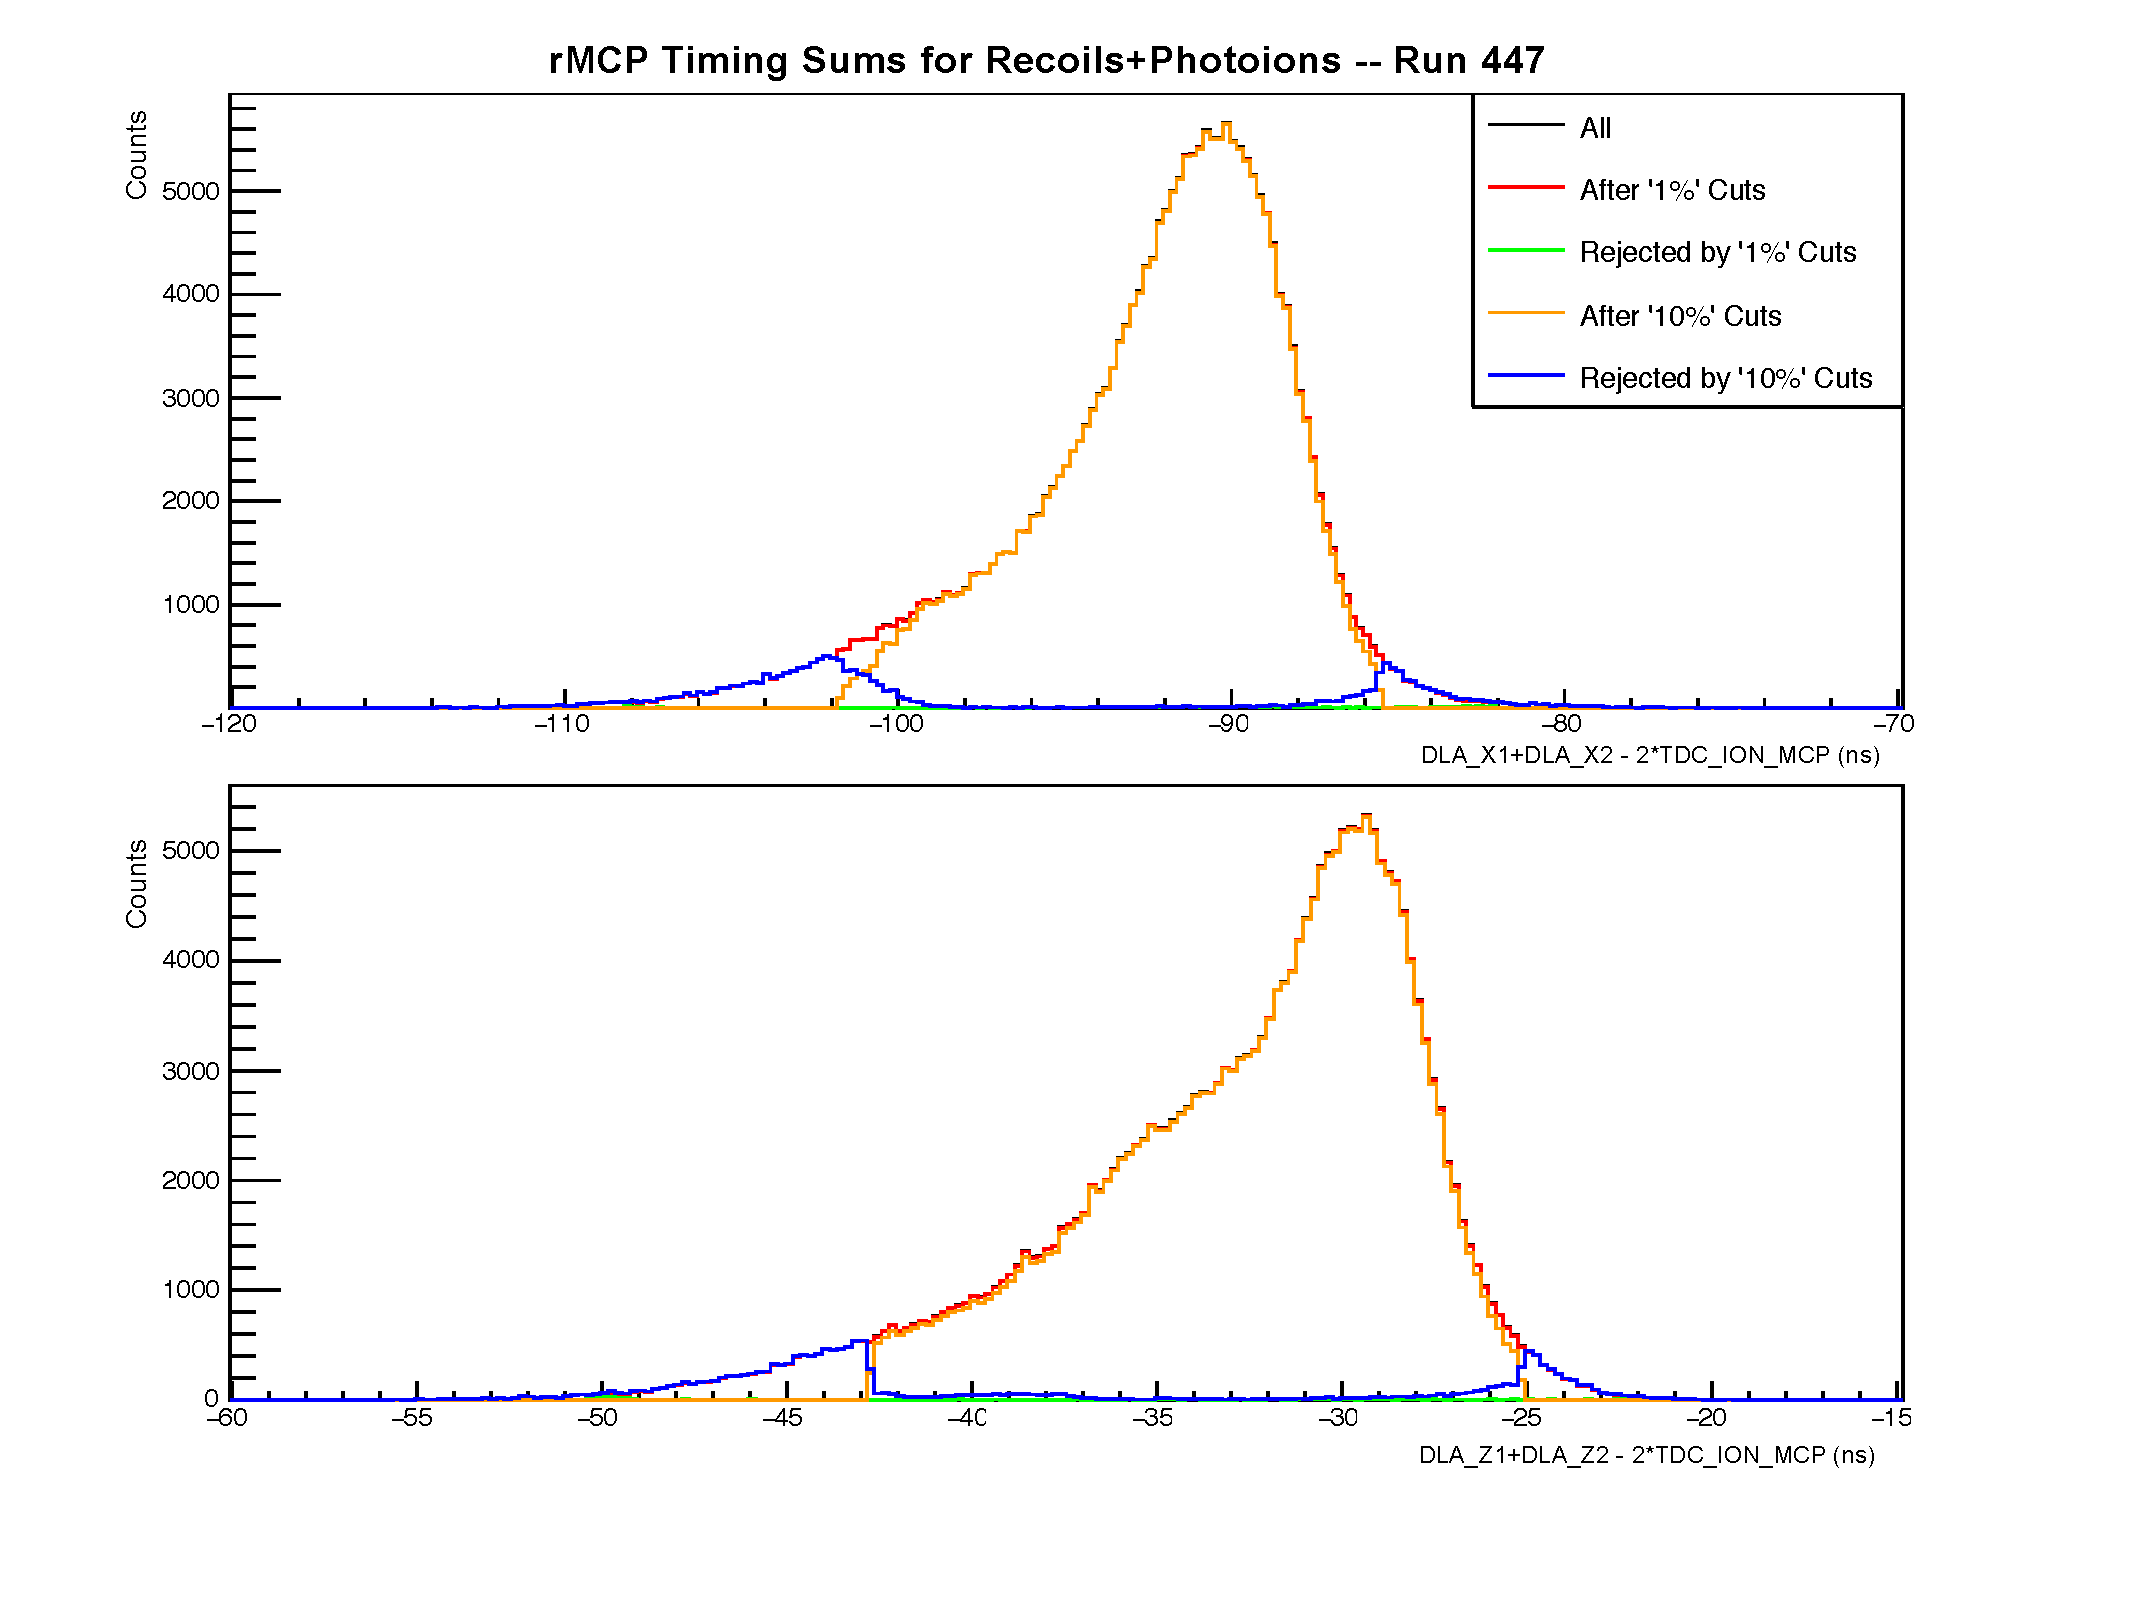
\includegraphics[width=.999\linewidth]
	{Figures/rMCP_sumcuts_447.pdf}
	\note{Are these things *definitely* in nanoseconds?  Check!}
%	\note{This algorithm does *not* discard $10\%$ of events!}
	\caption[Timing sums for the rMCP, run 447.]{Timing sums and associated cuts for the rMCP detector, run 447.  The `$10\%$' cuts shown simply eliminate events in which the distribution's height at that value is less than `$10\%$' of that distribution's maximum, and the `$1\%$' cuts are performed in a similar manner.  Note that this is \emph{not} the equivalent of eliminating $10\%$ ($1\%$) of events. The above distributions each show the results within their own distribution after cuts are taken on the \emph{other} distribution.  Only a single run is shown here to avoid washing out features -- because the characteristics of these spectra varied significantly over the course of the beamtime, and not all of the changes can be attributed to a change in settings.
	}	
	\label{fig:sumcuts}
\end{figure}

Because the characteristics of these timing sum distributions varied from run to run, it didn't make sense to aggregate all the data before taking cuts, so any cuts had to be chosen on a run-by-run basis.  Because of the asymmetry and occasional bimodality of the distributions, it also didn't make sense to try to fit the distributions to a function such as a gaussian and then cut away some number of sigma from the fit function.  The algorithm that was used in the end was to determine the peak's maximum, then discard events from the portion of the distribution in which the distribution's height is less than $10\%$ of the maximum.  Fig.~\ref{fig:position_with_sumcuts} shows the effect of these cuts on the measured cloud position within a single run.

\begin{figure}[h!tb]
	\centering
	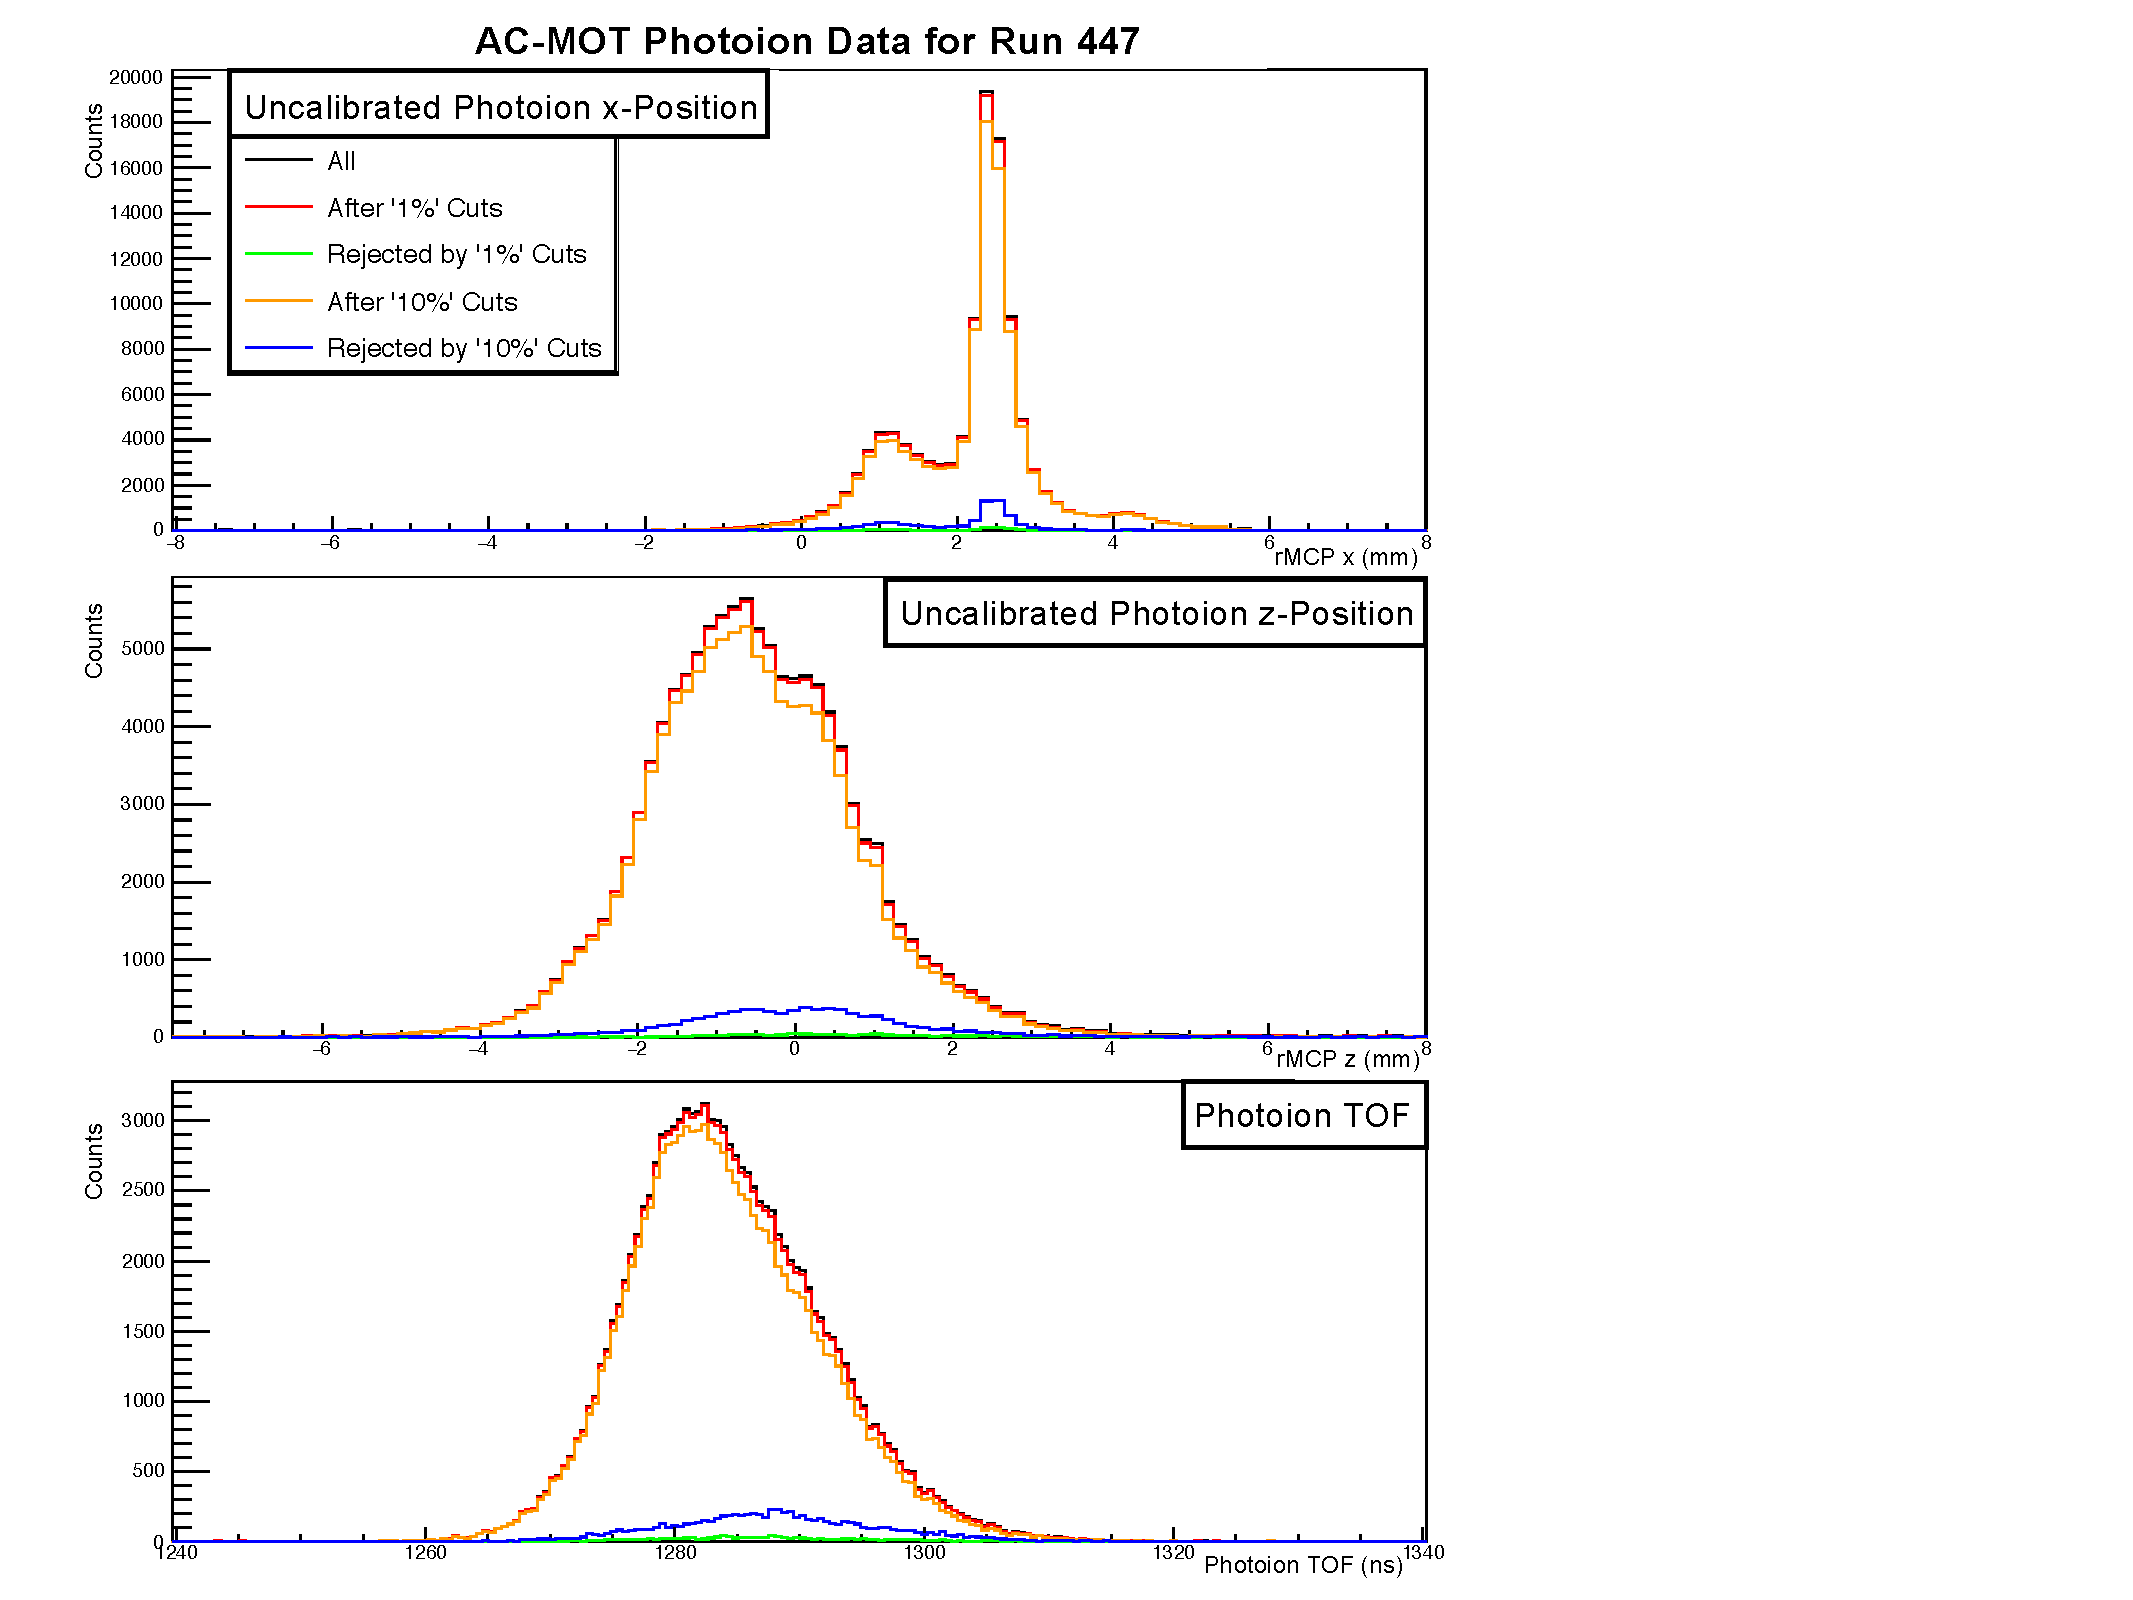
\includegraphics[width=.999\linewidth]
	{Figures/rMCP_xyz_comparecuts447.pdf}
%	\note{This figure needs to be discussed in text or whatever.}
	\caption[Cloud Position for run 447 for various rMCP timing sum cuts]{Cloud Position for run 447 for rMCP timing sum cuts as shown in Fig.~\ref{fig:sumcuts}.}	
	\label{fig:position_with_sumcuts}
\end{figure}

%-- so all cuts on the rMCP delay line timing sums had to be taken on a run-by-run basis, and because of the asymmetry and occasional bimodality of the distributions,   

\FloatBarrier  % I think this has to go away eventually.
\section{Calibrations with the rMCP}
\label{sec:rmcp_cals}
A calibration mask was created for the rMCP, to eliminate any nonlinearities in the images produced.  Several months before the $\isotope[37]{K}$ beamtime was to occur, the mask was attached in front of the rMCP, and a test of the delay lines' ability to produce an image was performed using an alpha source to illuminate the full surface of the detector.~\aside{I *think* we used an alpha source?  Not sure what else we could have done, but I better check this!}  The mask was later removed in advance of the beamtime, in order to preserve the highest possible surface area, and calibrations were performed using the older mask data and subsequently applied to the online $\isotope[37]{K}$ data.% (see Fig.~\ref{fig:rmcp_calibration}).

The calibration to the offline data with a visible mask was performed over a number of steps.  The data was given a preliminary rough calibration, performed on each delay line separately, which simply involved taking the difference in pulse arrival times between each end of the delay line, scaling the result by a factor chosen to get the image to be the approximate correct size, and then subtracting an offset to center the image.  

With the preliminary calibration providing a visible image to work with, the `$10\%$' cuts as described in Section~\ref{sec:rmcp_cuts} were applied, significantly sharpening the visual mask lines and overall image border. Next, a small rotation was applied, followed by a more precise centering algorithm. Following this, a linear stretching algorithm was applied to adjust the height and width of each row and column individually, while aligning the grid lines to their known position on the detector.  Finally, an additional radial stretch was applied to only the outer areas of the image.  This last adjustment can be justified by noting that it's expected for the outer parts of the detector to produce a more distorted image, and that appeared to be the case here.  See Fig.~\ref{fig:rmcp_calibration}.
%indeed the outer areas of the image did appear more `squished' relative to the rest.  See Fig.~\ref{fig:rmcp_calibration}.  

When the online rMCP data was eventually collected, it was found that the rMCP image appeared offset by several centimeters relative to the previous calibration, which necessarily affected the location of the timing sum peaks (similar to those shown in Fig.~\ref{fig:sumcuts}).  The most likely cause for this is a change in cable lengths between the readout and data acquisition in the months between the calibration and online data collection, but it meant a new set of `$10\%$' cuts needed to be established for the online data, and also cast some doubt on the validity of the established calibrations.  In the end, these cuts were established on a run-by-run basis due to the varying shape of the timing sum peaks.  

%In the end, a new set of `$10\%$' cuts was established for each individual run, since the peaks' characteristics seemed to change over time.  
Our ability to confidently accurately apply the old offline calibration to the new online data depended on our ability to center the image correctly, as different parts of the image are stretched and squeezed differently.  The appearance of the plate edge--the only remaining indicator of the quality of the centering or overall calibration--changed shape slightly from run to run.  Despite this, images from the online data were all summed together after applying run-by-run cuts, and the resulting image was centered by eye.  

The centering was performed iteratively, because the subsequent steps in the calibration will distort the image differently depending on how accurately it was centered beforehand.  These subsequent steps in which the image is stretched and squished will also change the apparent centering of the overall image.  Calibrated and uncalibrated images are shown in Fig.~\ref{fig:rmcp_calibration} for both offline and online data.

%it's necessary to perform the subsequent steps in the calibration 
%Therefore, a new offset had to be estimated by eye, then entered into the correct step in the calibration \emph{before} the stretching occurred.  Since the stretching algorithm itself changed the apparent centering too, this was an interative process.  

\begin{figure}[h!tb]
	\centering
	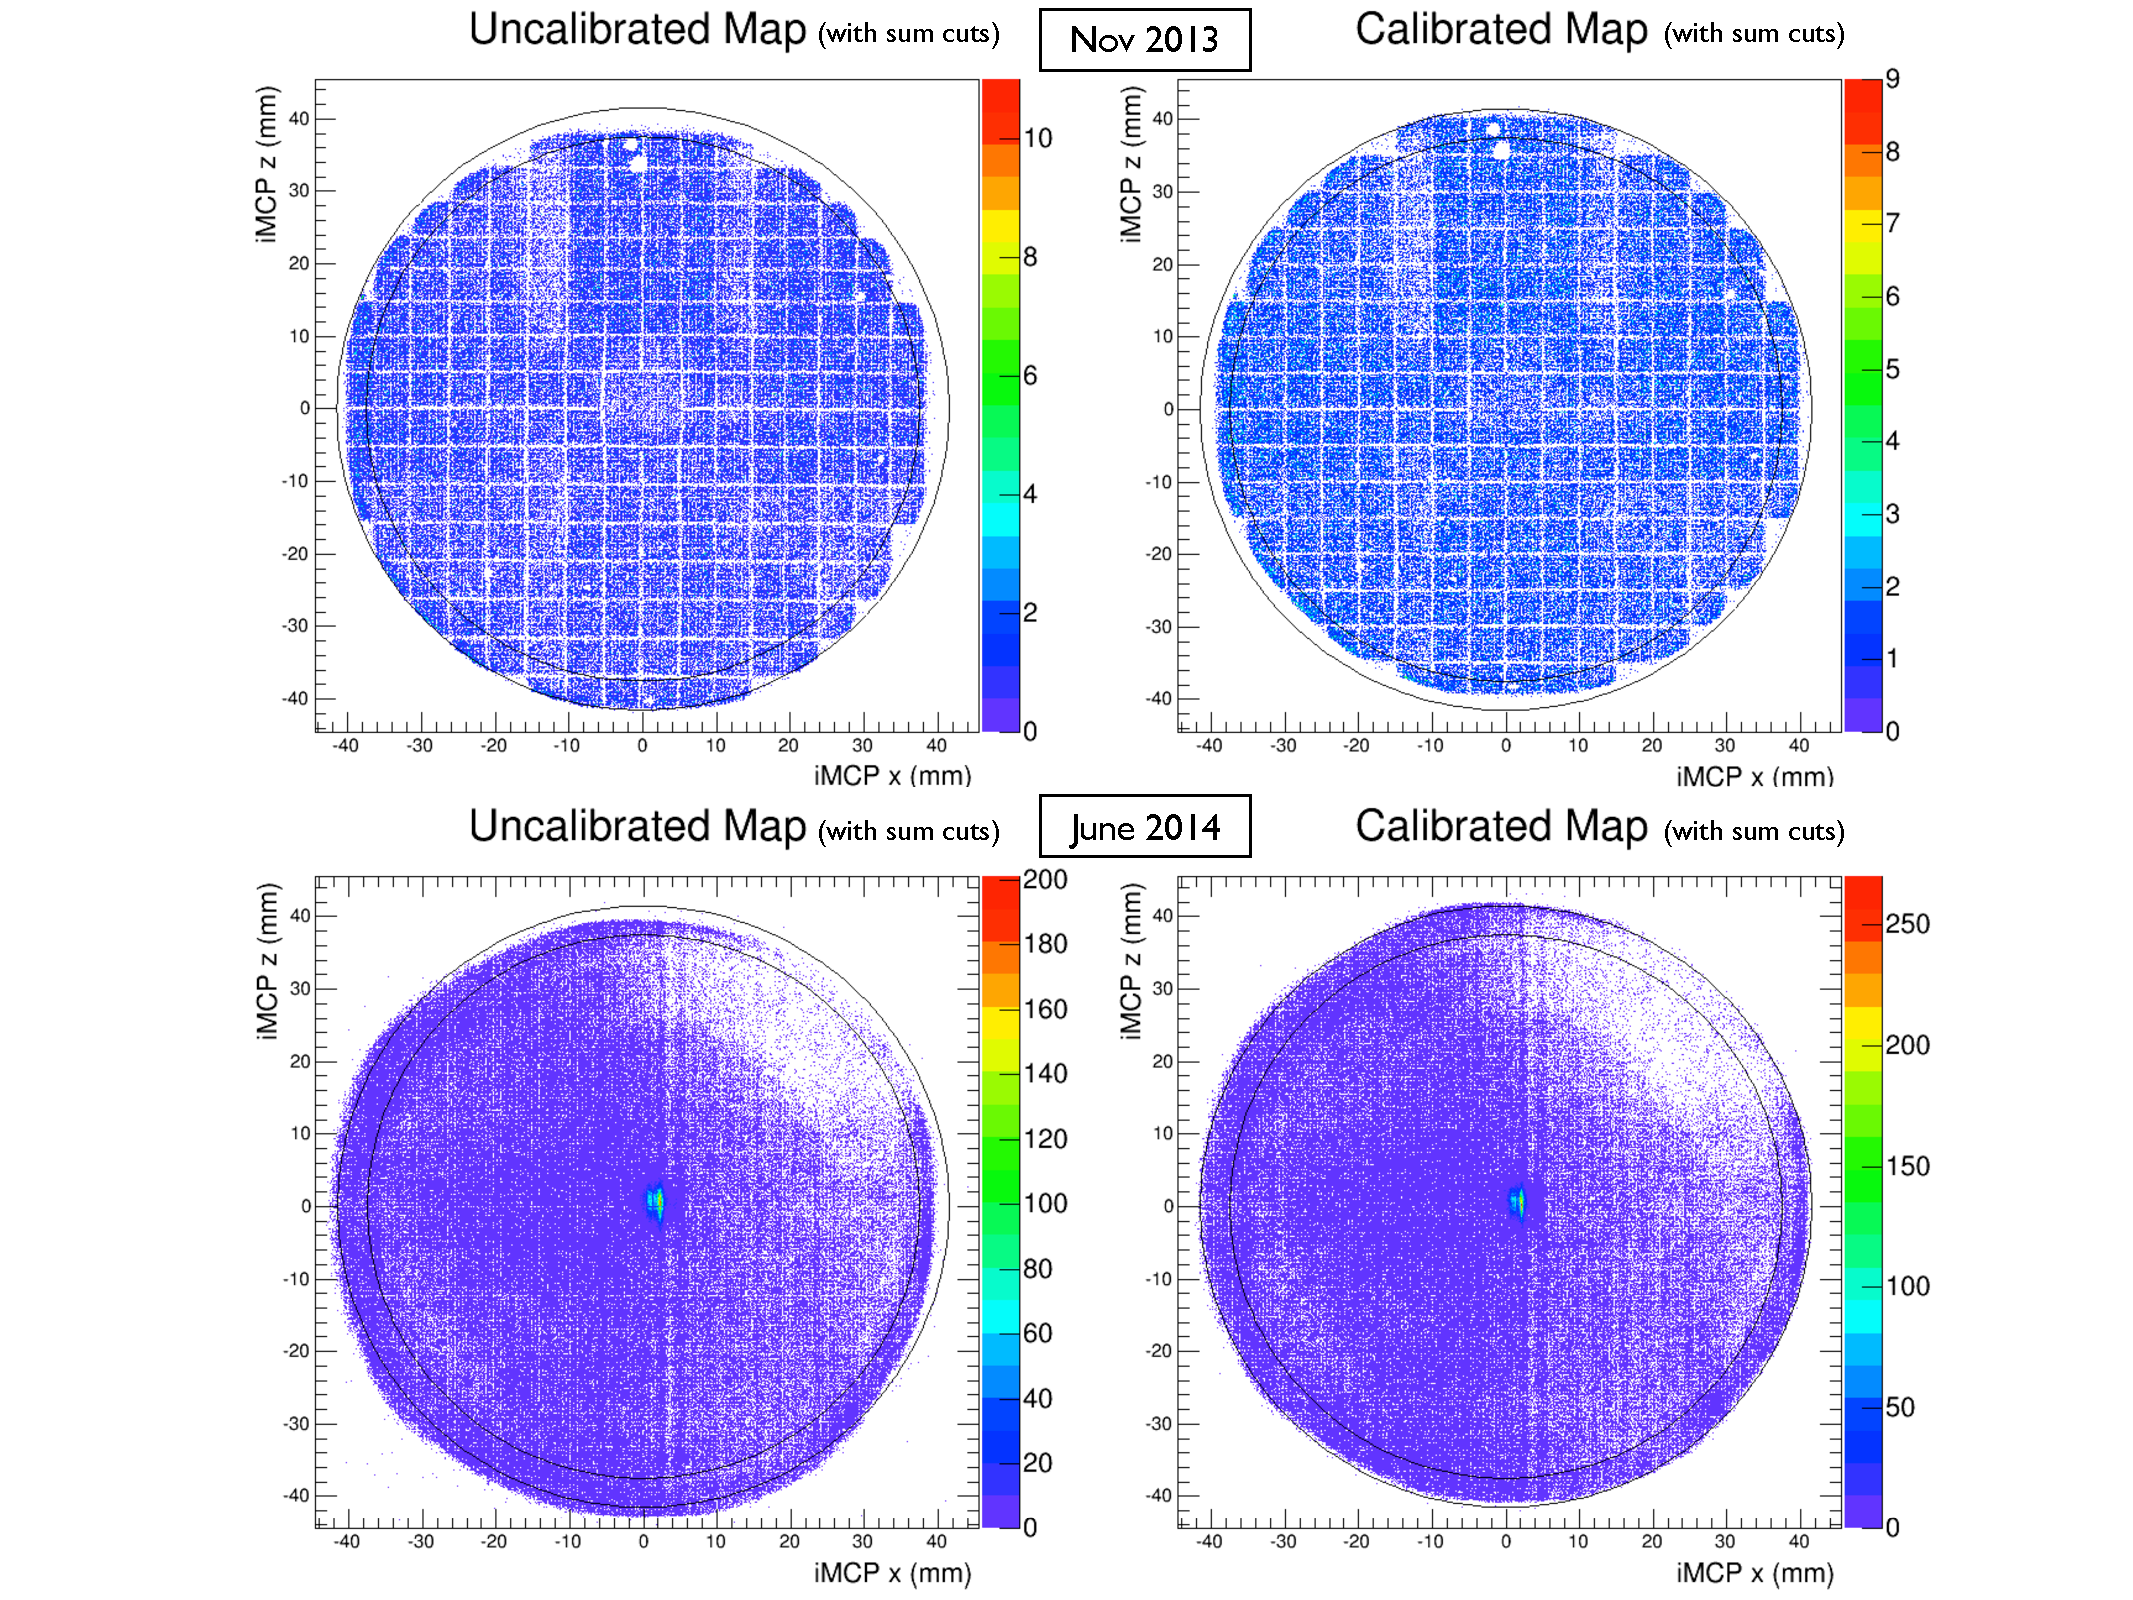
\includegraphics[width=.999\linewidth]
	{Figures/rMCP_Calibration}
	\caption[rMCP Calibration]{rMCP Calibration.  The left images show the rMCP hit map with only a basic preliminary calibration; the images on the right are filled with the same hit data, but after the calibration has been performed.  The upper two images are from data collected offline in advance of the 2014 beamtime using an alpha source; the shadow from a calibration mask is clearly visible.  The lower images show rMCP data taken from a single online run, and includes both photoion and nuclear recoil data, collected over both the polarized and AC-MOT times.  The photoion image of the atom cloud visible in the centre of the lower plots.}
	\label{fig:rmcp_calibration}
\end{figure}

The lower plots in Fig.~\ref{fig:rmcp_calibration} show an unfortunate pattern of vertical stripes across the full surface of the rMCP.  These stripes persisted over many (but not all) of the online runs.  They can still be clearly seen in Fig.~\ref{fig:photoionhits_2D}, which is a sum of all Runset RB's photoion events. The cause for these stripes could not be determined, and they could not be removed in post-processing analysis.  

\begin{figure}[h!tb]
	\centering
	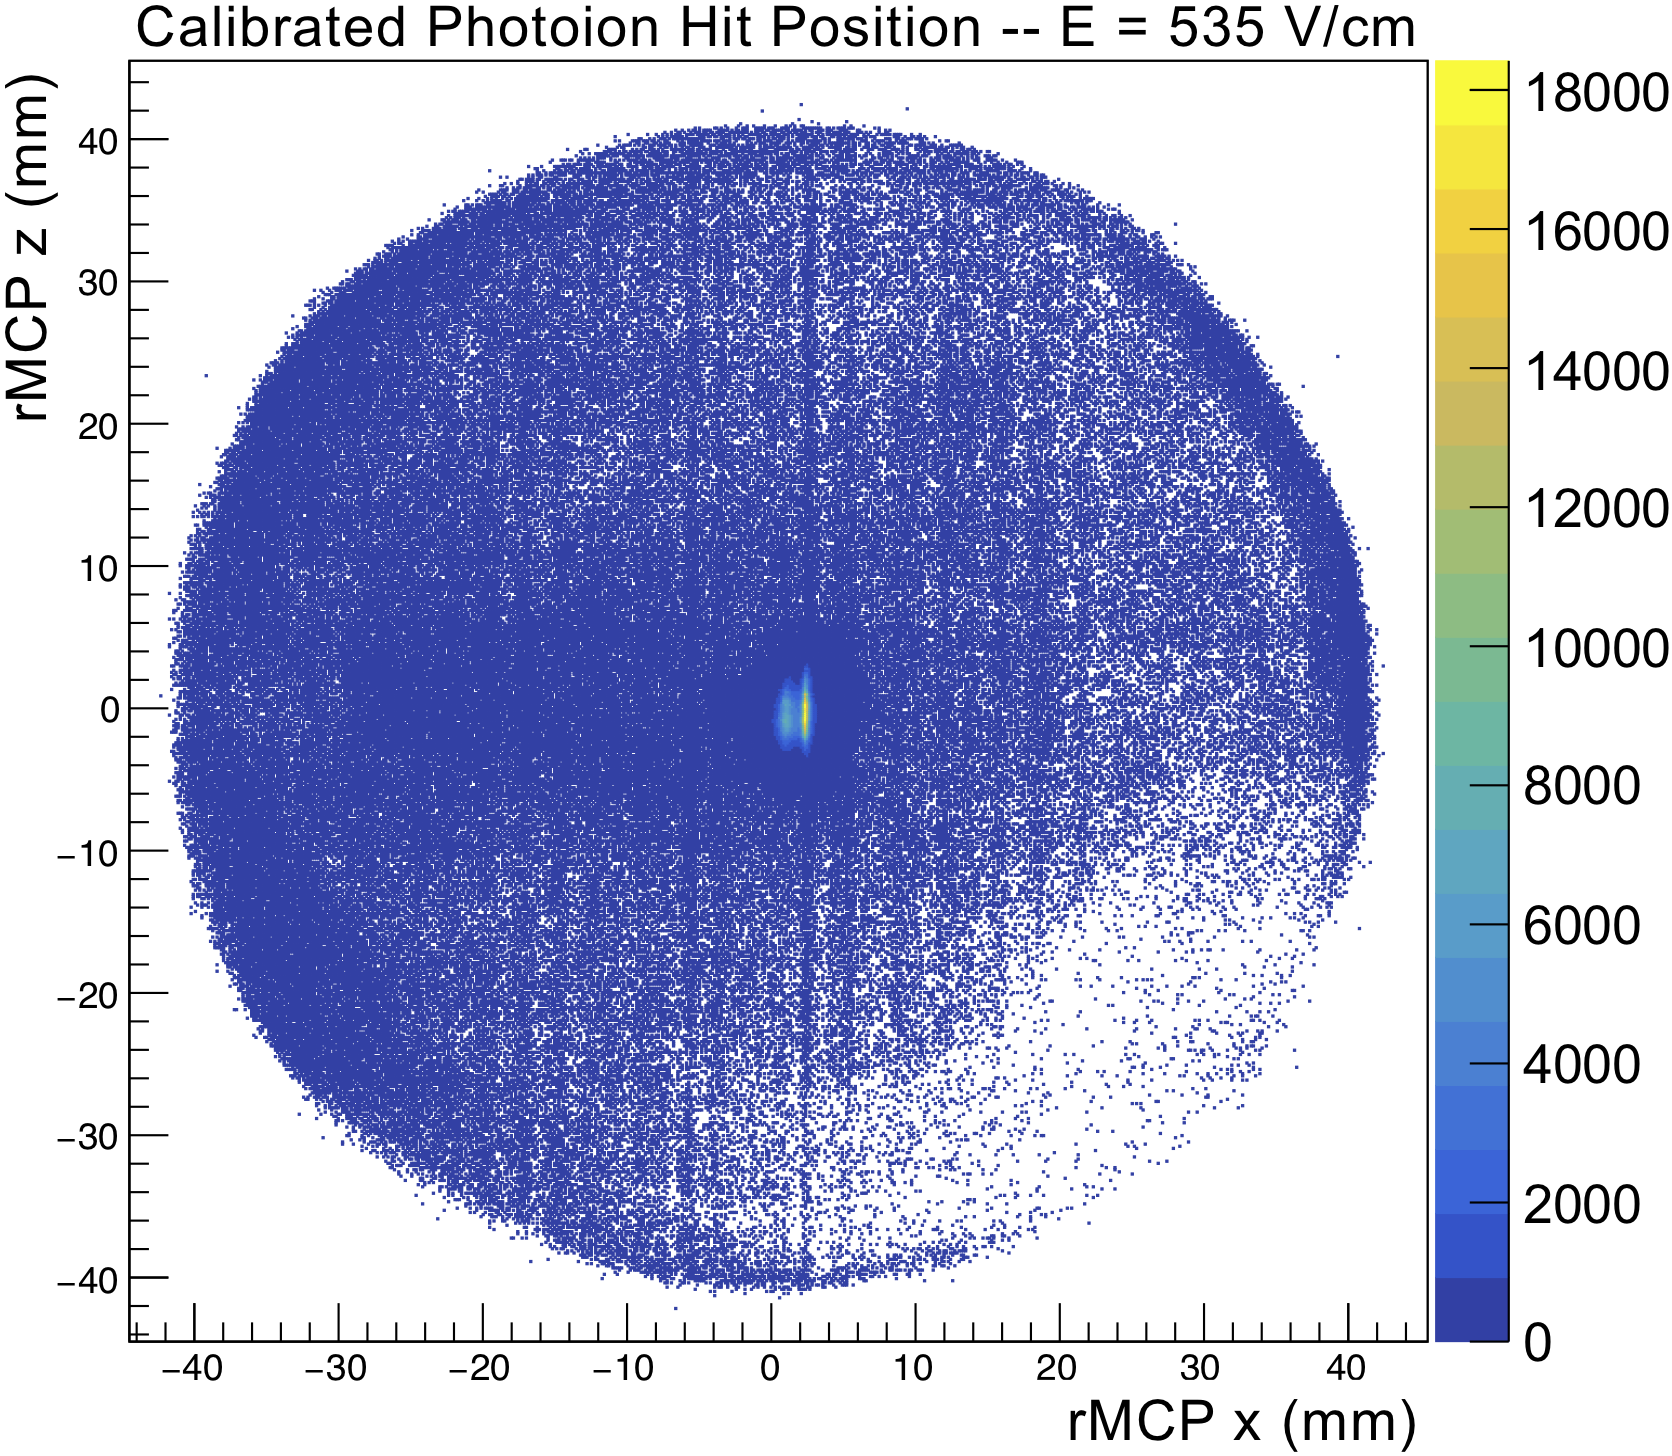
\includegraphics[width=.999\linewidth]
	{Figures/rMCP_PI_2D_535.png}
	\note[color=bluetodo]{You know, I think this one is flipped relative to the previous image.  Bleh.  Probably this one is the correct one, but who wants to deal with that?  Also .... did we switch MCP plates between calibration and the run?  I think possibly we did!  I'll have to ask the eLog.}
	\note{Does this thing even have a TOF cut?}
	\caption[Photoion Hit Positions in 2D]{Photoion Hit Positions in 2D.  This is the entirety of the good photoion data taken at 535 V/cm.  The central bright spot is an image of the atom cloud arising from photoionization events of unpolarized atoms; the rest is background.  Vertical stripes of indeterminate cause can be seen across the face of the image -- it has not been possible to eliminate them in analysis. %, and it is unclear what result they may have with regard to estimates of the average trap position and size.
	}	
	\label{fig:photoionhits_2D}
\end{figure}



\note{It is worth mentioning that the mask calibration data was collected without the presence of the magnetic fields involved in trapping and optical pumping, but these were of course present in the online data to which it was being compared.  Since a magnetic field can change the trajectory of a charged particle, one might suspect that there could be some effect on the resulting image.  There are two stages at which this might occur:  while the ion is accelerating through the electric field within the experimental chamber before impacting the rMCP, and while the electron shower is emerging from the back of the MCP stack before it is incident on the delay lines.  
...
But also, I really don't want to get into this, otherwise somebody will ask me to quantify the size of the effect.  Turns out:  it's tiny, but it will be really annoying to demonstrate that.}


%The calibration involved:
%\begin{itemize}
%	\item rotate
%	\item cal\_slide
%	\item big\_squeeze
%	\item micro\_squeeze\_x and micro\_squeeze\_z
%	\item edge\_stretch
%\end{itemize}

%\note{the rMCP does both cloud position *and* cloud polarization, and it collects data faster than the camera can go, so we really kind-of need it for polarization I think?  Except we had that oscilloscope readout too, and that would have basically been fine I think.  Camera does position, but not quickly, so we'd just get an average over all the AC-MOT times or whatever, which isn't really what we want.  Though, turns out that's not a super big systematic anyway.  But whatever, the rMCP is useful, dammit!}
%\note{ Using the ``other'' data set with the rMCP:  Measure the trap position/size/velocity/expansion with the rMCP and with the camera.  Necessitates calibrating the rMCP, which is its own whole thing.  Also measure polarization.}

%These calibrations are done during AC-MOT time (wait, is that even true?  I don't think so...), and we're actually interested in the rMCP data taken during OP time.  Can I find pictures to estimate the size of the change resulting from the magnetic field?  In any case, the change is pretty small.  

\FloatBarrier
\section{Measurements of the Atom Cloud}
\label{sec:cloud_calibration}
%\note[color=cleanup]{Write that final paragraph about measuring the atom cloud before and after OP.}
With the rMCP detector calibrated (Section~\ref{sec:rmcp_cals}), several types of data may be extracted.  It is possible to extract the hit positions and times-of-flight for the incident nuclear recoils, and an analysis of such data could be used to perform a test of right-handed currents within the nuclear weak force, as discussed in Chapter~\ref{section_rslow}.  However, we will focus here on what may be learned about the \emph{atom cloud} from rMCP events in coincidence with the photoionization laser.~\aside[color=org]{Also... does the camera data go in this section??}  

This class of data (events with both an rMCP hit and a photoionization laser hit in coincidence) can be used to measure cloud polarization, and the methodology and results of that process as it applies to this particular experiment are discussed in a recent publication~\cite{ben_OP}.  We are also interested in the cloud's position and size during the periods of time where decay data is collected, since this represents a potential systematic effect that must be accounted for within our models.  The latter will be the primary focus of this section.  

The first step in such a measurement is to try to eliminate as much background as possible.  We have already required that every event considered here must include both an rMCP hit and a photoionization laser pulse.  As we are interested in measurements of trap position, it makes sense to also require a \emph{complete} set of position data recorded on the rMCP's delay lines.   This is further trimmed by a `$10\%$ cut' on the timing sums, as described in Sec.~\ref{sec:rmcp_cuts}.  Any event including a scintillator hit is rejected, as these events have an increased likelihood for a recoiling ion to be detected on the rMCP instead of- or in addition to the photoion we expect (It is at this stage of the process that Fig.~\ref{fig:photoionhits_2D} is created.).  Finally, some fairly loose cuts are applied about the central x- and z-positions, as well as the ion's time of flight (measured with respect to the arrival of a photoionization laser pulse).

With these basic cuts performed, the cloud position and size must be measured.  We are particularly interested in measurements of the cloud during the time when it is considered to be \emph{polarized} --- however the great majority of photoionization events occur when the cloud is \emph{not polarized} (see Fig.~\ref{fig:position_v_acmottime_3axes}).  This is because the photoionization laser acts only on excited atomic states, which are readily available during the operation of the MOT.  When the MOT is shut off, the atoms quickly de-excite.  At the start of optical pumping 300$\,\mu$s later (in the case of the 535 V/cm data), there is a short burst of photoions due to the atoms being temporarily placed into an excited state as part of the optical pumping process.  The photoion burst falls away rapidly as atoms are optically pumped into the stretched state and can no longer be excited by the optical pumping laser.  

\begin{figure}[h!tb]
	\centering
	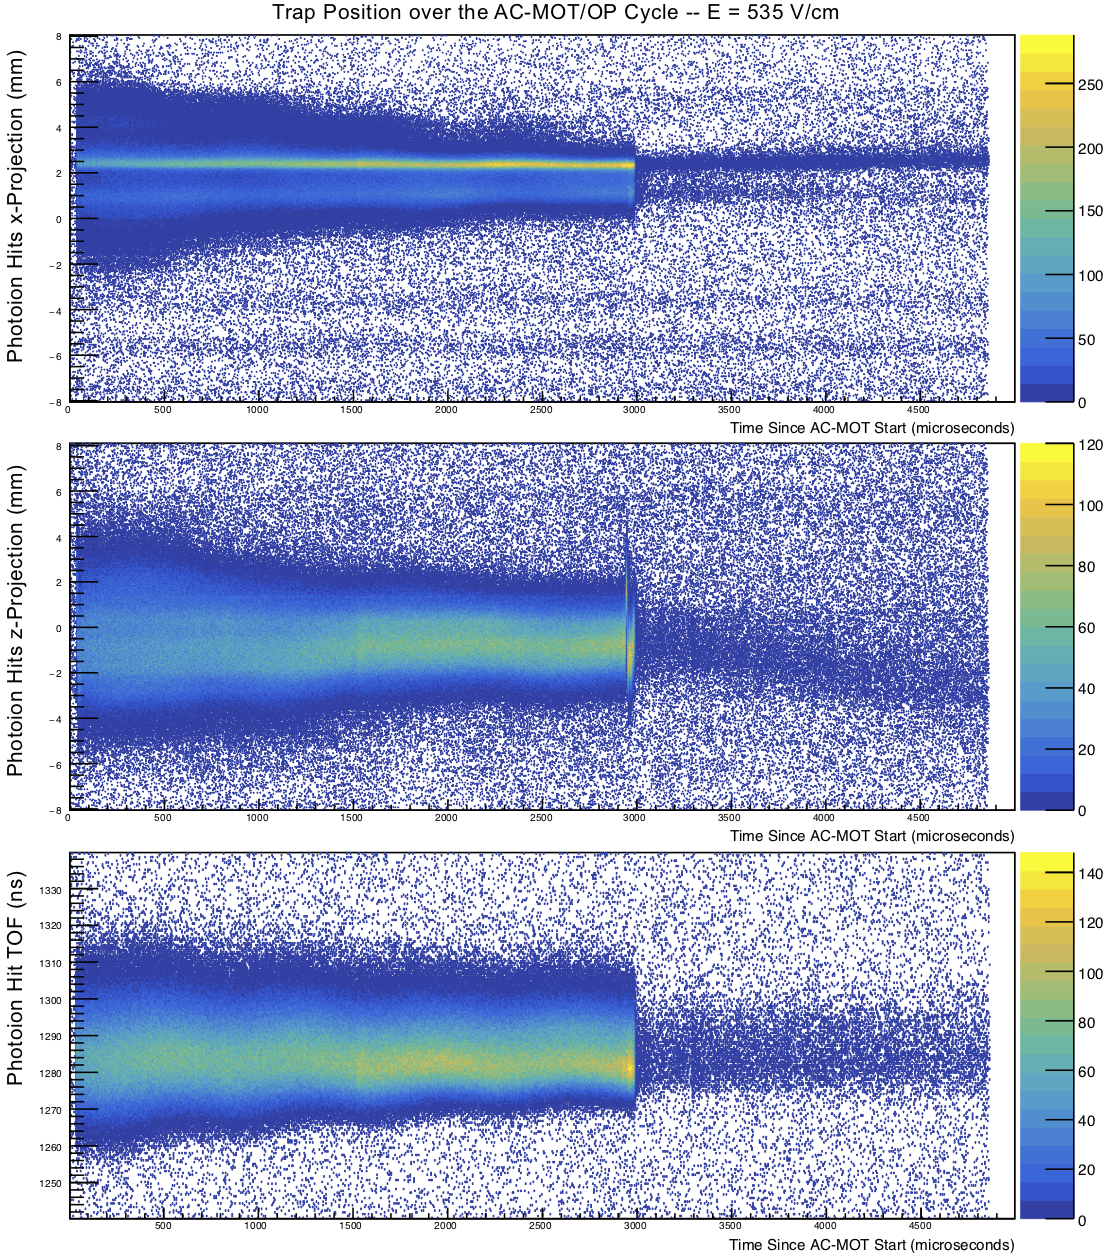
\includegraphics[width=.999\linewidth]
	{Figures/rMCP_xyz_vs_acmottime.png}
	\caption[Photoion Hit Positions at 535 V/cm, as a function of AC-MOT Time]{Projections of photoion hit positions and TOF at 535 V/cm, as a function of time since the start of the last AC-MOT cycle.  The trap's periodic motion can be seen in sync with the AC-MOT's cycles, and it is clear that the cloud is also being compressed during this time, before being allowed to expand ballistically when the MOT is shut off.  The photoion burst at the start of optical pumping 300$\,\mu$s after the AC-MOT is shut off can be seen on the lower two plots. 	}	
	\label{fig:position_v_acmottime_3axes}
\end{figure}

A projection of the cloud's position on the x- and z-axes, and its TOF (indicative of position along the y-axis) is plotted over the course of the repeating AC-MOT/OP cycle in Fig.~\ref{fig:position_v_acmottime_3axes}. The mysterious vertical stripes seen Fig.~\ref{fig:photoionhits_2D} are clearly evident in the top plot of Fig.~\ref{fig:position_v_acmottime_3axes}, and their positions do not change over the AC-MOT cycle, even though cloud motion is clearly visible.  
 
%With these basic cuts performed, the 
%may have also produced a recoiling ion which could be detected on the rMCP instead of- or in addition to the photoion we expect.  
%To that end, we immediately discard any event in which a scintillator recorded a hit 

%Anyway, here is a nice table describing the atom cloud, for each of 3 runsets, and I'll immediately reference it right now, as Table~\ref{table:cloudpositions}:
To extract the size and position of the atom cloud as projected onto all three axes, time slices of several hundred $\mu$s are taken from the beginning of the AC-MOT cycle, and from the part of the AC-MOT cycle immediately before the MOT is turned off.  A gaussian is fitted to the cloud projection, with its parameters describing the trap's size and position during these parts of the cycle.  A linear interpolation applied to describe the cloud's 3D size and position during polarized times, as functions of time since the AC-MOT cycle started.  Results are shown in Table~\ref{table:cloudpositions}.

%%\note{Trap position -- Measured using the same dataset that was used to quantify the polarization.  The trap drifts slightly over the course of our data collection.  Describe the rMCP calibration needed to extract this info.}

% !TEX root = ../thesis_main.tex


\begin{table}[h!!!!t]
	\begin{center}
	\begin{tabular}{ c | r || lcl | lcl || lcl | lcl |}
	%	\hline
	%		\multicolumn{5}{ | c | }{Cloud Measurements -- $x$-Projection} \\
	%	\hline\hline
	%	\cline{3-6}
			\multicolumn{2}{  c  }{ } & 
				\multicolumn{3}{  c  }{ \!\!Initial Position\!\! } &  \multicolumn{3}{   c  }{ Final Position } &  \multicolumn{3}{   c  }{ Initial Size } &  \multicolumn{3}{   c  }{ Final Size } \\
		%	\cline{2-6}
		%	\hline
		%	\cline{2-6}
			\cline{2-14}
			\multirow{3}{*}{Runset B}  & $x$ & \,\,1.77 & \!\!$\!\! \pm  \!\!$\!\! & 0.03   & \,\,2.06   & \!\!$\!\! \pm  \!\!$\!\! & 0.08    & 0.601 & \!\!$\!\! \pm  \!\!$\!\! & 0.013 & 1.504 & \!\!$\!\! \pm  \!\!$\!\! & 0.047 \\
								& $y$ & -3.51    & \!\!$\!\! \pm  \!\!$\!\! & 0.04   & -3.33     & \!\!$\!\! \pm  \!\!$\!\! & 0.05    & 1.009 & \!\!$\!\! \pm  \!\!$\!\! & 0.013 & 1.551 & \!\!$\!\! \pm  \!\!$\!\! & 0.018 \\
								& $z$ & -0.661  & \!\!$\!\! \pm  \!\!$\!\! & 0.005 & -0.551   & \!\!$\!\! \pm  \!\!$\!\! & 0.021  & 0.891 & \!\!$\!\! \pm  \!\!$\!\! & 0.004 & 1.707 & \!\!$\!\! \pm  \!\!$\!\! & 0.015 \\
			\cline{2-14}
			\multirow{3}{*}{Runset C}  & $x$ & \,\,2.22  & \!\!$\!\! \pm  \!\!$\!\! & 0.05  & \,\,2.33   & \!\!$\!\! \pm  \!\!$\!\! & 0.11    & 1.18   & \!\!$\!\! \pm  \!\!$\!\! & 0.04   & 1.538 & \!\!$\!\! \pm  \!\!$\!\! & 0.087 \\
								& $y$ & -3.68     & \!\!$\!\! \pm  \!\!$\!\! & 0.04  & -3.31      & \!\!$\!\! \pm  \!\!$\!\! & 0.06   & 0.965 & \!\!$\!\! \pm  \!\!$\!\! & 0.012 & 1.460 & \!\!$\!\! \pm  \!\!$\!\! & 0.030 \\
								& $z$ & -0.437   & \!\!$\!\! \pm  \!\!$\!\! & 0.09  & -0.346    & \!\!$\!\! \pm  \!\!$\!\! & 0.037 & 0.927 & \!\!$\!\! \pm  \!\!$\!\! & 0.007 & 1.797 & \!\!$\!\! \pm  \!\!$\!\! & 0.026 \\
			\cline{2-14}
			\multirow{3}{*}{Runset D}  & $x$ & \,\,2.274 & \!\!$\!\! \pm  \!\!$\!\! & 0.012 & \,\,2.46 & \!\!$\!\! \pm  \!\!$\!\! & 0.06   & 0.386 & \!\!$\!\! \pm  \!\!$\!\! & 0.016 & 1.382 & \!\!$\!\! \pm  \!\!$\!\! & 0.046 \\
								& $y$ & -4.54      & \!\!$\!\! \pm  \!\!$\!\! & 0.04   & -4.28    & \!\!$\!\! \pm  \!\!$\!\! & 0.04   & 0.986 & \!\!$\!\! \pm  \!\!$\!\! & 0.08   & 1.502 & \!\!$\!\! \pm  \!\!$\!\! & 0.013 \\
								& $z$ & -0.587    & \!\!$\!\! \pm  \!\!$\!\! & 0.04   & -0.481  & \!\!$\!\! \pm  \!\!$\!\! & 0.018 & 0.969 & \!\!$\!\! \pm  \!\!$\!\! & 0.003 & 1.861 & \!\!$\!\! \pm  \!\!$\!\! & 0.013 \\
			\cline{2-14}
	\end{tabular}
	\end{center}
%	\label{table:cloudpositions}
	\note{These positions are for the *electron* runsets of those names.  Might want a chart of which rMCP runs are used to measure position for which eMCP runs.  Possibly in that other section.}
	\note{Sig figs here need work.}
	\caption[Cloud Position and Size]{Cloud Positions and Sizes -- Measured immediately before and immediately following the optical pumping phase of the trapping cycle.  All entries are expressed in units of mm, and the ``size" parameters describe the gaussian width.}
	\label{table:cloudpositions}
\end{table}

  %  \label{table:cloudpositions}

\FloatBarrier %%% this will have to go.

\note{Also, we noticed the trap drifting after one of the runs, because one of the batteries on one of the thingies adjusting the laser frequency (I think) was failing. }
\note[color=jb]{JB:  ``If we rejected the data with the MOT moving (indeed a battery determining the voltage controlled oscillator frequency offset between absorption in stable \isotope[41]{K} cell and the \isotope[37]{K} resonance) then that's all you need to say.''}
\note{describe how you'd turn this into a physical description of the cloud, with like a temperature and a sail velocity and shit.  with equations.}


%I really need an excuse to include more pictures of data.  Also, more pictures of simulations.
%Without further ado, I'm just going to put in several pictures.  Right here, right now.  They're likely to *actually* show up on subsequent pages mixed in with the other content.  I'll have to fix that at some point.

%%%%%%\note[color=tag]{Get rid of at least like two out of the three stupid camera plots.}
%%%%%%\begin{figure}[h!!t]
%%%%%%	\centering
%%%%%%	\includegraphics[width=.999\linewidth]
%%%%%%	{Figures/y_from_camera_electron_recoil.pdf}
%%%%%%	\caption[Trap Position along TOF Axis]{Trap Position along the ``Time-of-Flight'' Axis.  Electron runs and recoil runs plotted by run number. \comment{(I should probably re-plot this.  Maybe combine info with Fig.~(\ref{fig:cameraposition_by_time}).) } }	
%%%%%%	\label{fig:camera_electron_recoil}
%%%%%%\end{figure}
%%%%%%
%%%%%%\begin{figure}[h!!t]
%%%%%%	\centering
%%%%%%	\includegraphics[width=.999\linewidth]
%%%%%%	{Figures/TrapPosition_FromCamera.pdf}
%%%%%%	\caption[Trap Position from Camera]{Trap Position along the ``Time-of-Flight'' Axis and the ``Vertical+30" Axis.  All runs plotted by time of run. \comment{(Need to re-plot this.)}}	
%%%%%%	\label{fig:cameraposition_by_time}
%%%%%%\end{figure}
%%%%%%
%%%%%%
%%%%%%\begin{figure}[h!!t]
%%%%%%	\centering
%%%%%%	\includegraphics[width=.999\linewidth]
%%%%%%	{Figures/VerticalTrap_by_rMCP_prelim}
%%%%%%	\caption[Vertical Trap Position from rMCP]{Trap Position along the Vertical Axis, plotted as a function of time of run (top) and run number (bottom).}	
%%%%%%	\label{fig:vposition_by_run_rmcp}
%%%%%%\end{figure}
%%%%%%


%%% !TEX root = ../thesis_main.tex
%%%
%%%
%%%
%%%%%% --- * --- %%%%	
%%\section{Data Selection and Preliminary Cuts Mini-Intro from John}
\FloatBarrier
\section{Electron Run Data Selection and Preliminary Cuts}
\label{sec:preliminary_cuts}
%\note{We now consider how to clean up our data.  We make some fairly obvious, intuitive cuts, and those are described here.  Later, we'll make less intuitively obvious cuts.}
%
%
%%%%Although the detection chamber was designed to feature two MCP detectors on opposing sides of an applied electric field intended for simultaneous use (see Section~\ref{section:mcps}), in practice the two detectors produced quite a bit of feedback when operated at the same time.  In order to salvage usable data from the beamtime, we ended up running only one detector at a time, but switched which detector was in use every few hours, collecting approximately the same amount of data with each detector.  Thus, the runs are sorted into `electron' and `recoil' runs, depending on what the detector in use was intended to detect.  
%%%%
%%%%While the beta asymmetry and Fierz interference are best evaluated using the electron runs, the recoil runs are best for evaluating the polarization (a dominant uncertainty in the beta asymmetry measurement) and the cloud position.  The polarization measurement is the subject of a recent publication (see~\cite{ben_OP}), and the cloud position evaluation is discussed in more detail in Chapter~\ref{calibrations_chapter}.
%%%%
%%%%The data is further split up into four runsets:  A, B, C, and D based on when certain detection settings were adjusted, and each of these runsets contains both electron and recoil runs.  These four runsets were then treated separately for nearly all parts of the analysis.  In particular, Data Set A was neglected completely during analysis after it was determined that one scintillator had an improperly set hardware threshold such that lower energy betas weren't being detected at all.  Additionally, there was a QDC module failure between Runsets B and C, resulting in an abrupt change in calibration for the two scintillators.  
%%%%\note{`The observant reader may find it curious that the listed runsets start at ``B'' and continue alphabetically.  There was initially a ``Runset A'' collected as well, however it was determined later that this data could not be salvaged for use in the final analysis because one of the scinitillators had its hardware threshold set above the compton peak, and without that reference point an accurate calibration could not be performed.'}
%%%%
%%%%%\note{Also, the background was too noisy in Set A I think.  Also, pretty sure there isn't really that much data in Set A at all.  Also-also, Set A has E=66.7, so can't use it for more stats on the other backgrounds. ... Maybe I should just look up what the deal even was with Set A, since I don't really remember.} 
%%%%
%%%%%\note{What did I change between Runsets B and C?  Between Runsets C and D?  ...OP time, yes, but also and one point a PMT(?) (eta:  it was a QDC) blew out and we replaced it, so then the scintillator calibration was a bit different afterward.  Anyway, I should maybe just make a goddamn table.  Table goes here.}
%%%%
%%%%% !TEX root = ../thesis_main.tex


\begin{table}[h!!!!tb]
	\begin{center}
	\begin{tabular}{ c || p{1.2cm} | r | l | p{5.8cm} | }
		\multicolumn{4}{l}{Electron Runs} %& \multicolumn{1}{l}{Electron Runs} 
		\\
		\cline{1-3}
		\multicolumn{5}{c}{ }
		\\
			\multicolumn{1}{  c  }{ } & 
				\multicolumn{1}{  c  } { \!\!OP Delay\!\! } &  \multicolumn{1}{ c }{ \!\!Events\!\! }  
				& \multicolumn{1}{ c }{ \!\!Electric Field\!\! } & \multicolumn{1}{ c }{ Runs } 
				\\
			\cline{2-5}
			\multirow{1}{*}{Runset A}	& $300\,\mu s$
										& 0
										& \,\,\,$66.67$ V/cm
										& 314, 362, 363, 383-386, 393. %, 420.
										\\
			\cline{2-5}
			\multirow{1}{*}{Runset B}	& $300\,\mu s$
										& 173,640
										& $150.0$\,\, V/cm
										& 428-437, 440-445.
										\\
			\cline{2-5}
			\multirow{1}{*}{Runset C}	& $700\,\mu s$
										& 18,129
										& $150.0$\,\, V/cm
										& 476, 477.
										\\
			\cline{2-5}
			\multirow{1}{*}{Runset D}	& $400\,\mu s$
										& 207,596
										& $150.0$\,\, V/cm
										& 478-489, 502-505, 510, 513.
										\\
			\cline{2-5}
	\end{tabular}
	\end{center}
	\note{A list of 2014 online runs with potentially usable data.  Runset A was discarded completely due to problems with hardware threshold settings.  There was a QDC module failure before Run 450, so it and all subsequent runs were performed using a different module, and as a result the scintillator calibrations changed slightly at this time.  Anyway, the point of this thing is to show which electron runs and recoil runs go together, for the purposes of evaluating polarization and cloud attributes.}
	\note{Ben doesn't seem to include Runs 436 and 437 in *any* set of good runs.  Is it an oversight?  I think they're perfectly legit electron runs.  They're fairly long runs...}
	\caption[List of Electron Runs]{A list of electron runs and associated parameters.  The ``Events'' column includes only the number of events that passed all cuts.}
%	\note{This table might eventually go away.  Mostly I just want a record of the total `good' counts.  In total, $N=399,365$.}
	\label{table:runlist_electrons}
\end{table}


%%%%% !TEX root = ../thesis_main.tex


\begin{table}[h!tb]
	\begin{center}
	\begin{tabular}{ c || r | l | p{7.8cm} | }
		\multicolumn{3}{l}{Recoil Runs}
		\\
		\cline{1-3}
		\multicolumn{4}{c}{ }
		\\
			\multicolumn{1}{  c  }{ } & 
				\multicolumn{1}{  c  } { \!\!OP Delay\!\! } 
				& \multicolumn{1}{ c }{ \!\!Electric Field\!\! } & \multicolumn{1}{ c }{ Runs } 
				\\
			\cline{2-4}
			\multirow{1}{*}{Runset RA}	& $300\,\mu s$
										& 395.0 V/cm
										& 303, 308-313, 318, 326, 327, 328, 340, 342, 343, 
										376, 377, 378, 394, 395, 396, 398-402.
										\\
			\cline{2-4}
			\multirow{1}{*}{Runset RB}	& $300\,\mu s$
										& 535.0 V/cm
										& 409-419, 421-426, 446, 447, 449.
										\\
			\cline{2-4}
			\multirow{1}{*}{Runset RC}	& $700\,\mu s$
										& 395.0 V/cm
										& 450, 454, 455.
										\\
			\cline{2-4}
			\multirow{1}{*}{Runset RD}	& $700\,\mu s$
										& 415.0 V/cm
										& 460-466, 473, 474.
										\\
			\cline{2-4}
			\multirow{1}{*}{Runset RE}	& $400\,\mu s$
										& 415.0 V/cm
										& 491, 497, 498, 499, 509. 
										\\
			\cline{2-4}
	\end{tabular}
	\end{center}
%	\note{This table might eventually go away.  Mostly I just want a record of the total `good' counts.  In total, $N=399,365$.}
	\note{Ben includes 448 as a `good' recoil run.  But I don't.  Why?  Also 451, 451, 453.  ...Also 467,468,469,470,471,472.  Also-also, 492, 493, 494, 495, 496.}
	\caption[List of Recoil Runs]{A list of 2014 online recoil runs and associated parameters.  A count of good events that pass all cuts is not included because different cuts must be used for polarization and trap position data.}
	\label{table:runlist_recoils}
%	\note{I really need to merge the two tables.  :(  ...also, add a new table to show which things should be used with which other things.}
\end{table}



Before proceeding further, several basic cuts are performed on the data.  For the Electron Runs which are to be processed directly into a physical measurement, we consider only events in which there was a recorded hit \emph{both} on the eMCP \emph{and} on exactly one of the scintillators.  The required scintillator hit, of course, is potentially a beta, and so it is obvious why this must be present.  Events in which both scintillators record a hit are discarded, as they fall into two categories:  an accidental coincidence, where we are seeing two different decays that, by chance, both occurred within the time window allocated to a single event (a few $\mu$s before and after the first recorded scintillator hit), a backscatter event in which a beta was incident on one scintillator before being scattered out into the opposite scintillator.  Although it would be possible to process the former event type into usable information if we could be certain that it was truly an accidental coincidence, contamination from the latter event type would serve to increase the systematic uncertainty arising from beta scattering--already a dominant source of error.\aside{Point at that other conclusion-ier section.}

%Geant4 simulations have shown that the latter event type is very uncommon, but scattering events
%and Geant4 simulations have shown that the latter event type is very uncommon, the latt
%events in the latter 

The eMCP is used primarily to record incident shake-off electrons.  As described in Section~\ref{section:soe_intro}, every beta decay event will produce one or more SOEs.  Most (but not all) SOEs originating from the atom cloud will be incident on the eMCP, 
%and these will arrive within a particular time window with respect to the scintillator hit time -- 
however not all incident SOEs on the eMCP will produce a recorded hit.  The electric field is such that SOEs originating elsewhere within the chamber may or may not be incident on the eMCP.  Therefore, while imposing an eMCP hit requirement will eliminate some `good' events originating from the cloud, it also eliminates a much larger fraction of background events originating from other surfaces within the chamber.  This ability to `tag' good events originating in the cloud is absolutely essential to any analysis involving angular correlations within this geometry.


In later sections, we will consider how to evaluate a further cut to be imposed on the time difference between scintillator and eMCP hits (Section~\ref{section:emcp_cuts}), and some subtleties within analysis relating to this choice (Sections~\ref{sec:bs} and~\ref{sec:tof_bg}).

%discuss further cuts using the eMCP data 
%In subsequent sections, we will discuss further cuts to be taken using the eMCP data (
% and so the eMCP hit requirement is an absolutely essential prerequisite to any analysis involving angular correlations within decay products in this geometry.  
%The eMCP hit requirement -- particularly with the timing of the eMCP hit occuring within a certain time range relative to the scintillator hit -- is used to tag beta decay events originating from the cloud, as opposed to those originating from some other surface within the chamber.  The eMCP typically records incident shake-off electrons,  
%A hit to the eMCP is typically a shake-off electron from a decay, however not every 

%Although at least one SOE is generated for every decay, no
%Most (but not all) of these SOEs will be swept to the eMCP by the electric field 
%\aside{Do I *ever* describe how this even works?  Where do we get the SOEs from?? }  
%The precise time interval to be used, and how it should be evaluated,\aside{also discussed: how we decide what counts as an eMCP hit at all} is discussed in Section~\ref{section:emcp_cuts}, and some subtleties within the analysis relating to this choice are considered in Sections~\ref{sec:bs} and~\ref{sec:tof_bg}.  
%Nevertheless, this cut must be made essentially at the beginning of the analysis in order for much of the rest to be internally consistent.
%, but for the first pass through the data it is good enough to simply require that an eMCP hit occurred.\aside{Awkward stupid phrasing.}  
%Although not every beta decay event from the cloud will produce a hit on the eMCP, this requirement eliminates a great deal of background that would otherwise be challenging to evaluate.  
%\aside{Also, we claim that it doesn't bias the data.  Much.  Didn't I try to evaluate how much it biased the data at one point?}  

%Because the eMCP hit is required as a `tag' of good events, i
It is also necessary to remove from direct consideration any event which is coincident with a pulse from the photoionization laser.  When photoionization occurs within the atom cloud, an orbital electron is removed from the atom and will be accelerated by the electric field into the eMCP, just as a shake-off electron from a decay would be.  If, by chance, this photoelectron arrives in coincidence with a scintillator hit, it would be interpreted as a decay event from the trap -- unless we preemtively discard it.  

Over the course of the runtime, there were several instances where we noted an apparent electrical discharge within the experimental chamber, producing enormous backgrounds for a short time.  The detectors typically recovered quickly afterward, so it was neither necessary nor useful to stop an entire run to wait for the system to recover.  Instead, the time when the discharge occurred was recorded, and events within approximately one minute of the spark time were discarded.  

We use only the ``fully polarized'' events for which we have a detailed understanding of the nuclear polarization (described in more detail in ~\cite{ben_OP}).  This means we must use \emph{only} events from the ``optical pumping'' portion of the duty cycle (see Fig.~\ref{fig:dutycycle}), and discard events when the DC- or AC-MOT is active.  After the AC-MOT is shut off, there is a short delay before optical pumping begins (see Tables~\ref{table:runlist_electrons} and~\ref{table:runlist_recoils}) to allow the magnetic field to decay, and it is only after $100\,\mu s$ of optical pumping that we consider the atoms to be fully polarized.  Furthermore, because the magnetic field from the DC-MOT is slow to decay (relative to the field from the AC-MOT), all events from the first five AC/OP cycles after every atom transfer are discarded.  A further benefit of our insistence on considering only polarized data is that the scintillators' gains are more stable in the presence of only the (small, stable) magnetic field used for optical pumping than they are in the presence of a larger oscillating magnetic field used for trapping~\cite{ben_thesis}.
\note{change by 0.2\% of its value vs change by 0.5\% of its value, according to Ben's thesis pg 143.}
\note{Ben didn't do the 5 cycle discarding thing in his Abeta analysis, but he *did* do it in his OP analysis.}

Finally, because this analysis depends heavily on energy measurements from the two scintillators as a proxy for beta energy, it is necessary to remove events in which the pulser LED fired.  Although the pulser LED is useful for evaluating the stability of the scintillators, in the case where an LED pulse occurs together with a true beta hit in the scintillator, it may change the measured energy.  Therefore, we discard all events that include an LED pulse.   
	


%\section{Beta Detector Cuts}
%	Setup is as described in Section~\ref{section:betadetectors}.	 
%	\note{This is a stupid section name.  Also, I really do need to describe how the cuts were made here somewhere, because it's non-trivial in many cases, and possibly different than what Ben did in some cases.  But it won't make sense to describe what I did different if I don't describe the thing as a whole, at least a bit.  The point is, this is a set of cuts/systematics that isn't really that straightforward to understand.  }
%\section{Plastic Scintillators}
%	\note[color=org]{Maybe this goes in Chapter~\ref{dataselection_chapter}?}
%	\note{Energy calibration for the scintillator+PMT setup changed dramatically at one point.    Describe how calibration was done.  Like, one sentence or something.  Something about the endpoint energy, and something about the compton edge for 511s, IIRC.}

\section{Further Cuts Using the DSSD}
%\note[color=org]{Pretty sure I'm repeating myself from Chapter~\ref{???}}
\note{Add 2D DSSD plots?}
\note[color=jb]{JB says: To repeat a comment, since the Appendix on analysis changes is being dispersed throughout, when you state somewhere (I think it's in Ch. 6)((5?)) make sure you state clearly that the only change for BB1 cuts
is the radius cut, e.g. that you took the same T and E from the waveforms (I'm not even sure whether the
waveforms are recorded anyway). You  ask 'how can I state this' but there's no reason to be subtle.
Just say upfront that Ben and Spencer's theses did all the groundwork on the BB1, and here you include selected details needed to understand the present analysis. If you need to include some redundant material, don't worry too much about that.
\\ ... \\ 
MJA:  In fact, I think the BB1 radius may have been the same.  The uniform energy threshold was different though.  But I get the point.
\\ ... \\ 
Also, yes, the waveforms are absolutely recorded in the MIDAS files but they haven't been saved to modern ntuples, because they made the files huge.  I think it's probably pretty easy to switch that on/off in the Analyzer though to generate a set of ntuples that has that info included.
}

\missingfigure{Show individual beta energy spectra.  ...with a variety of different cuts, perhaps?}


Although it was not possible to use the DSSD in real-time analysis or event triggering, the DSSDs may be used, after the data has been collected, to distinguish between different types of particles incident on the detector, as more energy will be deposited by heavier particles.  When a scintillator hit is triggered by a particle originating within the experimental chamber, that particle will typically have passed through the DSSD before arriving at the scintillator.

In the present experiment, the two primary particles that will concern us are $\beta^+$ particles originating from the decay of $\isotope[37]{K}$, and $\gamma$ rays, which may be produced through a variety of processes, e.g. directly from the $2\%$ decay branch, through annihilation of $\beta^+$ particles upon their interaction with regular-matter electrons, or bremsstrahlung radiation from emitted $\beta$s.  

We would like to look specifically at events involving $\beta^+$ particles arriving direct from a decay within the atom cloud, and the DSSD may be used to eliminate events in which the scintillator is triggered by a $\gamma$.  An incident $\beta$ will typically deposit some portion of its energy in the DSSD as it passes through, however an incident $\gamma$ will deposit significantly less energy; for this setup the energy deposited by a $\gamma$ is generally indistinguishable from background on the DSSDs.  Therefore, we require that a `good' event must include a `good' hit to the DSSD as well as a hit to the associated scintillator.   

In order to proceed at this point, and because the DSSD readout records so much information, it is necessary to develop some criteria to determine whether or not we will accept any given DSSD readout as a $\beta$ hit.

\note{How do I *say* that Ben was the one who did most of the DSSD calibration stuff?  I maybe don't need to describe all of it here, but I *could*, and maybe it's needed in order to understand like 4 rows in my error budget.}  

\note[color=jb]{JB:  ``You can describe anything you did differently or improved, but you can and should otherwise defer all details of the scintillator calibration and DSSD calibration to Ben's paper and his thesis and Spencer's.  E.g. Section~\ref{section:bb1_systematics} ``statistical agreement between BB1 X and Y detectors' energies only makes a small effect on results" does not need the technical details beyond that statement.''
\label{thesisconventionjb} }
\note[color=jb]{JB:  ``If you have some way of documenting the coding you used, that would be great.''  ... yeah, it would, wouldn't it?}


We read out the full waveform for every strip at each event with a scintillator hit, but in post-processing take \emph{only} the `time' and `energy' from the peak waveform height and the time in the waveform at which that occurs. Each strip will have its own noise spectrum and energy calibration.  To classify an event as a good DSSD hit, we require at least one `x' strip and one `y' strip record an energy above the noise threshold.  We require that the x strip and the y strip agree (to within some number of standard deviations) in amount of energy deposited, and in the time at which that hit occurred.  In order to avoid problems resulting from the strips' non-uniform noise thresholds, we further require that the energy deposited be greater than some lower-end cutoff which is selected so as to be higher than every individual strip's noise threshold.  In this case, the DSSD's lower energy uniform threshold was set at 50 keV.  

\note{I think Ben might have selected 60 keV?  That's maybe something for the appendix.}

We also elect to use only events where a beta hit the DSSD within a $15.5\,$mm radius of the center of the detector, so as to avoid scattering effects from the collimator walls. \aside{Did I even mention the collimator?  Like, in the previous chapter or something..?}

%Look at all the events to determine how noisy each individual strip is.  Do that for all strips.  Is the energy higher than some noise threshold?  by like a few sigma?
\note{Also-also (did I mention it already?) look for events with only *one* DSSD hit (two could indicate the beta scattered back out of the detector in another pixel, or alternately an accidental coincidence of two beta decay events.  either way, no good for analysis.)  Also, only one scint hit, and it has to be the on the same detector with the DSSD.   (...A scintillator hit as indicated by a TDC readout, as well as a max. recorded scint energy for the ``extra'' scintillator at something stupidly tiny, like 10 keV.  Probably *actually* 10 keV.) }

\note{After all other cuts -- not before!! -- we eventually use only events with scint energy between 400 - 4800 keV.  High cutoff is because of the low number of events, which makes the observable--the superratio asymmetry--poorly defined and poorly behaved.  Low cutoff is because it's really hard to model what's going on down there to the required level of precision.  The observable depends most heavily on low beta energy events, so it is imperative that the lower energy portion of the spectra be thoroughly understood if they are to be used for analysis. }
\note{Somewhere I should list what the energy cutoff is for this spectrum.  Or semi-equivalently, the Q-value.}






% % % % %%% % %%% % % % %
%\section{Further Cuts Using the eMCP}
\section{Timing Improvements with the Leading Edge and Scintillator Walk Correction}
\label{section:emcp_cuts}
\note[color=jb]{MJA:  I can describe the eMCP calibration here, even though it mostly wasn't implemented by me.  It is tangentially relevant to data selection and background estimation by providing an experimental energy spectrum for shake-off electrons.  It's actually a pretty neat algorithm that I basically wasn't involved with.
\\...\\
JB:  eMCP.  You need to describe the timing information obtained.  You also need a statement of whether or not you used the position information in your cuts.
\\...\\
MJA:  Wait.  So have I done that yet in this section?}

\note[color=org]{I described the HEX-75 somewhere in a previous chapter, right??}
\note[color=org]{I dislike how this section is organized..  should discuss the cut we *didn't* make at the end.}
%\note[color=org]{Really, should title this section according to the LE thing that is actually its primary topic.  In practice, the change only gets used on the SOE TOF cuts though.}
%Much like the rMCP, the eMCP is backed by a set of delay lines for position sensitivity.  .......
The eMCP features a set of three delay lines, intended to be used to record the position of a hit, as in Fig.~\ref{fig:emcp_position}.  \aside{Do I need to describe MCPs and delay lines somewhere?  Maybe not...}  Though only two delay lines is sufficient to determine the position within the plane of the MCP if they are both hit, the presence of a third delay line allows for some redundancy.  In practice, however, a large fraction of otherwise `good' events include a hit on the eMCP, but have insufficient information recorded on the delay line channels to reconstruct a position.  

\begin{figure}[h!!!!t!]
	\centering
	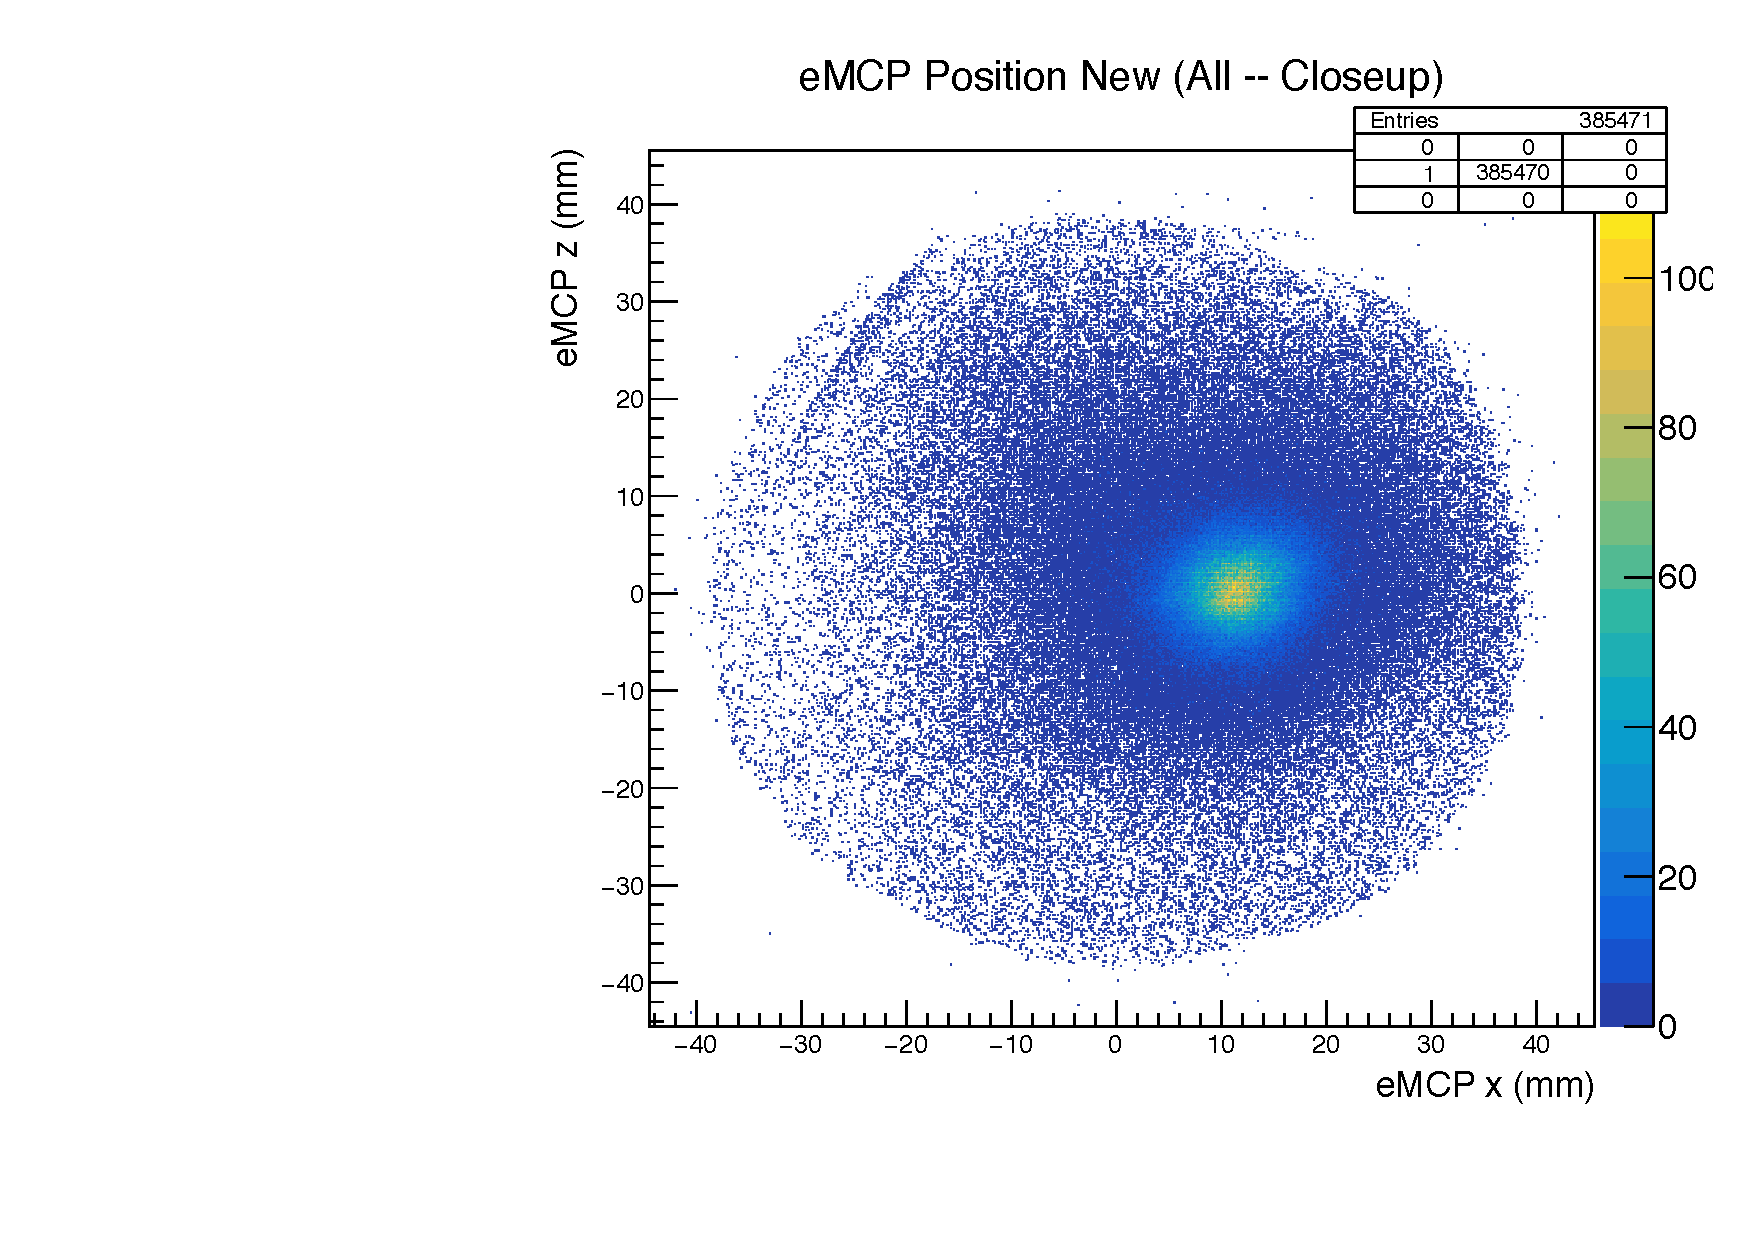
\includegraphics[width=.999\linewidth]
	{Figures/eMCP_position.pdf}
%	\note{This picture is `slow'.  Need to re-save it as a png.}
	\note[color=org]{This pic is probably better used in an SOE section somewhere.}
	\caption{Position as measured on the eMCP, after some data cleaning.}	
	\label{fig:emcp_position}
	\note[color=tag]{Delete eMCP image, or possibly move to the intro to describe Levinger.  Otherwise I have to talk about it here.}
\end{figure}

Because a SOE from the trap is most likely to land in the centre of the plate, while the background from other sources is roughly constant across the plate, \aside{Wait, what?} it might make sense to accept only events where the eMCP hit is within some radius of the central peak.  This methodology was seriously considered because the remaining data has a much lower fraction of background events polluting it -- however this results in a loss of around half of the events even for the most generous eMCP radius cuts (see Fig.~\ref{fig:soe_tof_positioncompare}).  Therefore, it was decided that no position cuts on the eMCP would be made in the final analysis.

\begin{figure}[h!!!!t!]
	\centering
	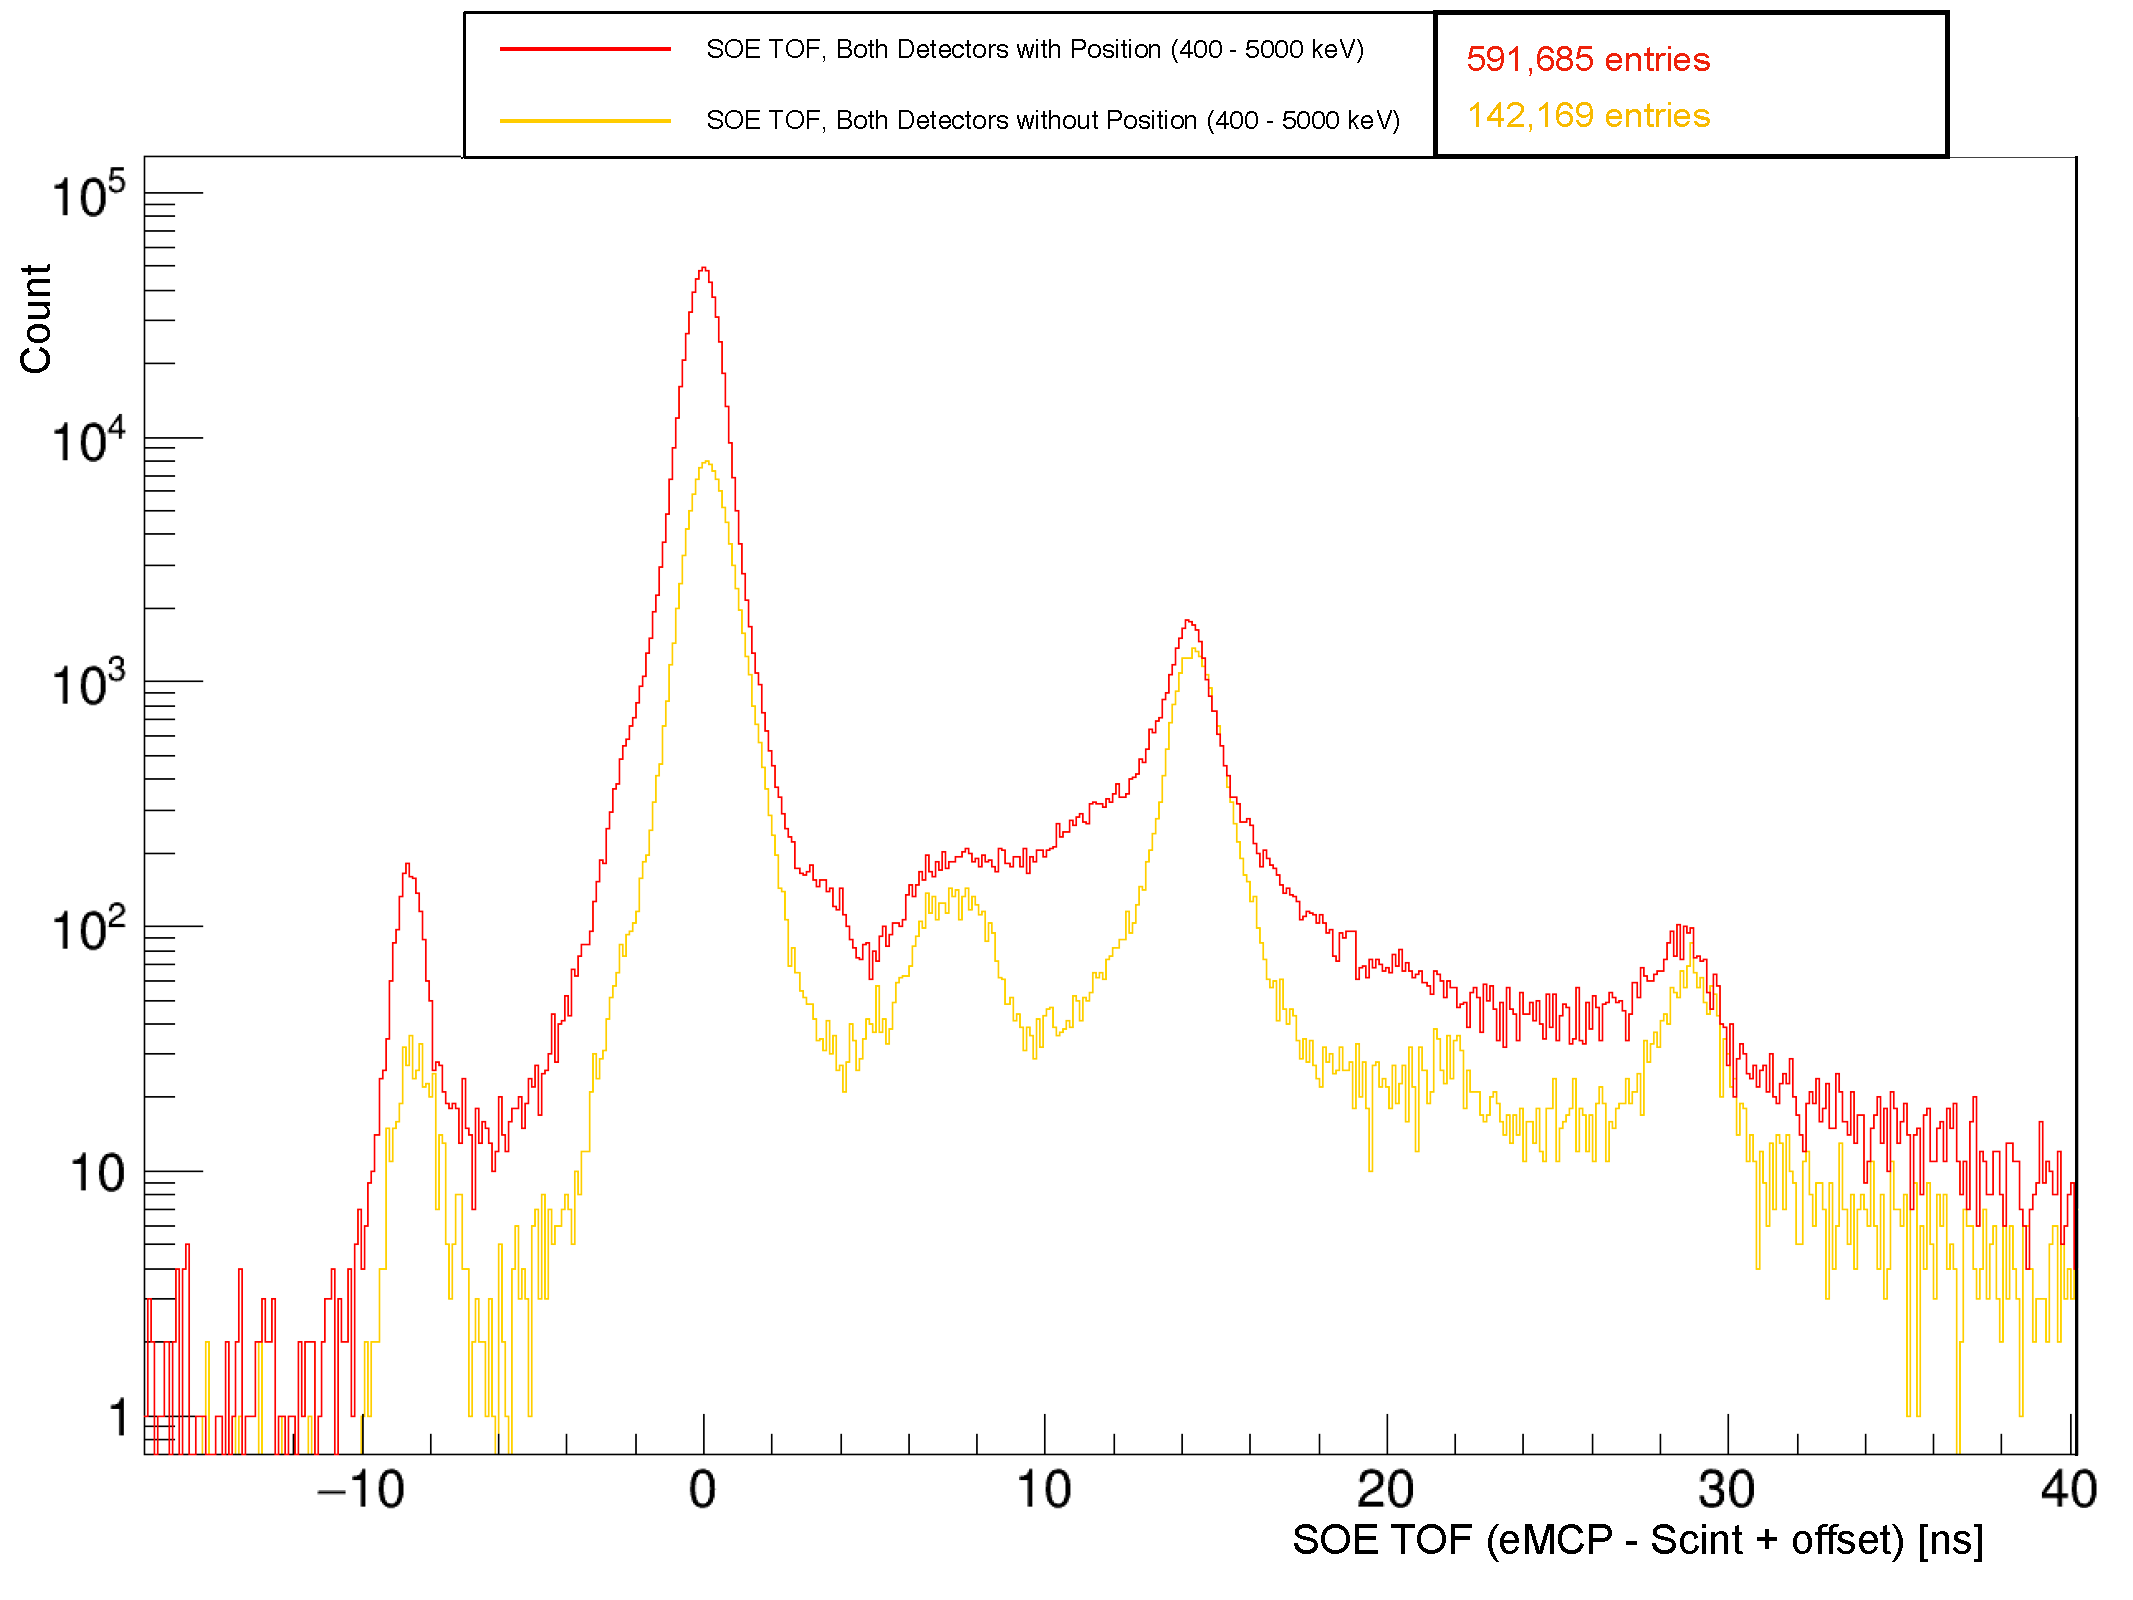
\includegraphics[width=.999\linewidth]
	{Figures/SOE_TOF_positioncompare.pdf}
	\note{Um.  Did I for sure get the labels correct on this???  It seems really wrong.}
	\note[color=org]{Surely this thing goes somewhere else instead.}
	\caption{Beta-electron TOF, for events with and without eMCP hit position information.  A cut will eventually be taken to accept only events sufficiently near the largest peak -- in this case the number of events is `only' decreased by a factor of 2.}	
	\label{fig:soe_tof_positioncompare}
	\label{fig:experimental_soe_tof}
	\note[color=tag]{Get a better set of experimental SOE TOF with/without position plots.  I think this one is wrong.}
\end{figure}

Several years after the data was initially collected, a problem was discovered with our low-level analyzer software, which we had been using to convert large and unwieldy MIDAS data sets into somewhat smaller and more manageable ROOT data sets.  In particular, for every timestamp recorded, our raw MIDAS data actually included both a timestamp for the leading edge (LE) of the pulse, and a timestamp for the trailing edge (TE).  The analyzer had--for years--been reporting the timestamp associated with the trailing edge of the pulse.  Initially it was unclear if there might have been a reason behind this choice, but a closer examination of the data showed that the LE data included less timing jitter and noise, as well as a sharper peak for timing pulses across the board (as in Fig.~\ref{fig:LE_TE}), with some channels showing a larger effect than others.  This was corrected, and the entirety of this analysis has been performed now using the cleaner LE spectra.  

\note{The LE spectra allows for us to use a more precise model of the SOE TOFs, so that's nice.}

\begin{figure}[h!!t!]
	\centering
	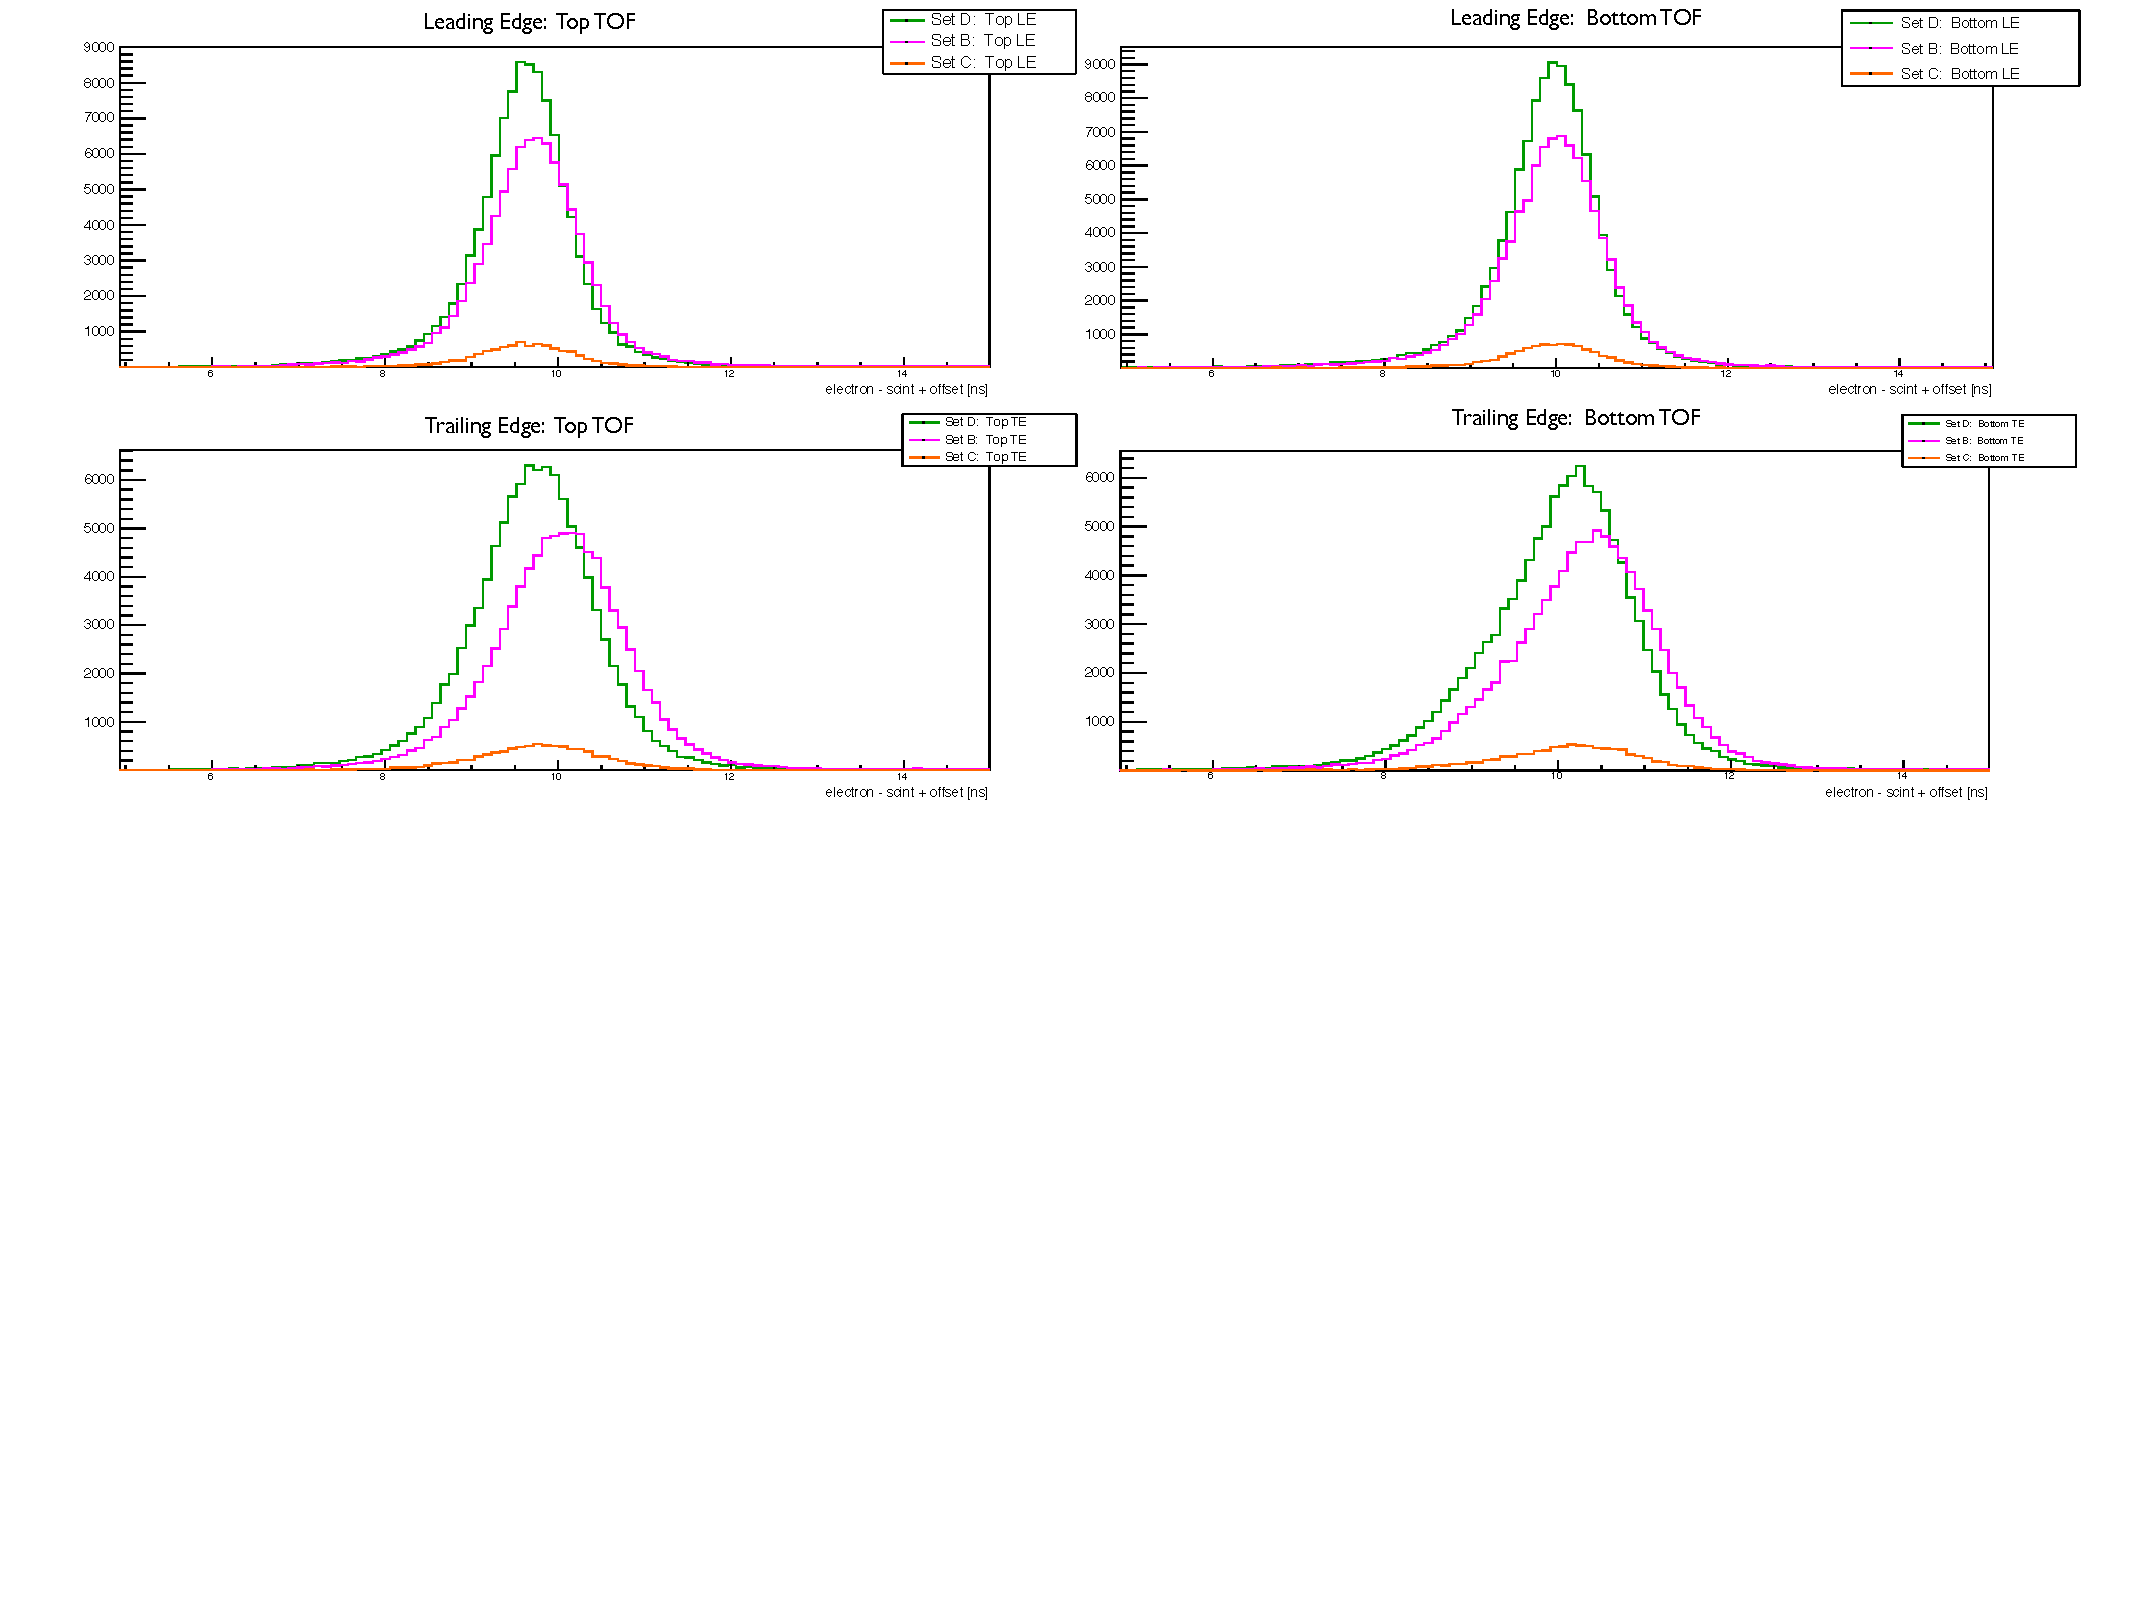
\includegraphics[width=.999\linewidth]
	{Figures/LE_TE_peaks.pdf}
	\caption{SOE TOF peaks (eMPC - Scintillator), using the leading edge (LE) and using the trailing edge (TE).  Data is sorted according to runset.  For each individual runset, the TE peak is broader than the LE peak.  The centroid of each runset is also more variable in the TE plots.}	
	\label{fig:LE_TE}
\end{figure}

The place where this change between the TE and LE timestamps had the biggest impact on the analysis is in the shake-off electron time-of-flight spectra, on which a cut must eventually be taken. Although this problem was not discovered in time to be used in the previous measurement of $\Abeta$ using this same data~\cite{ben_Abeta}, it likely would have had a negligible effect on the final result, because the SOE TOF cut that was used there was comparatively loose, and the evaluation of the background that remained was not a dominant systematic effect. \aside[color=org]{This goes in that one appendix, if I haven't already put it there.  ...Also, is this even fucking true?!?}

With the data reprocessed using the leading edge for timestamps, I wanted to eliminate as much background as possible from the SOE TOF spectrum.  With this goal in mind, the next step was to correct the scintillator timing for its low energy `walk' (see Fig.~\ref{fig:WalkAdjust}).  A quartic polynomial was fit to each of the 2D timing vs energy spectra (the top and bottom detectors were treated separately), and the result was used to produce a `straightened' SOE TOF spectrum with respect to measured scintillator energy, and as expected, the resulting SOE TOF spectrum was a bit more sharply peaked.  


\begin{figure}[h!!!!tb]
	\centering
	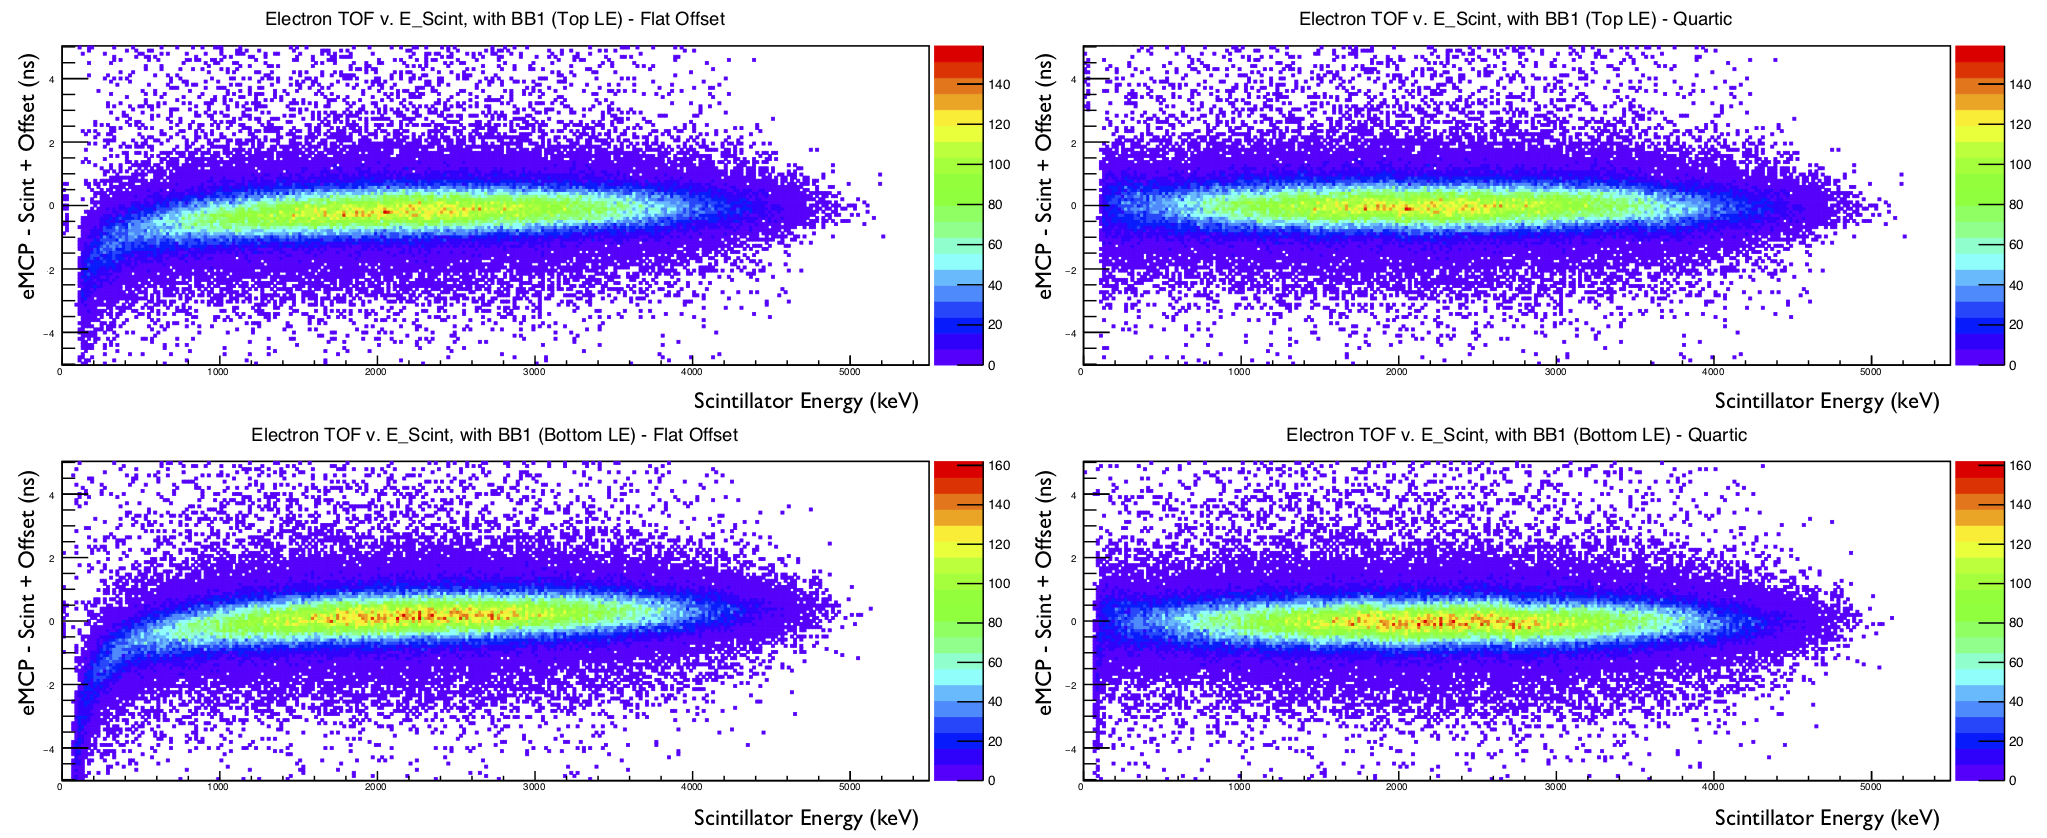
\includegraphics[width=.999\linewidth]
	{Figures/WalkAdjust.png}
	\caption{SOE TOF walk, before (left) and after (right) applying a quartic adjustment to straighten out the effective TOF.}	
	\label{fig:WalkAdjust}
\end{figure}

With the SOE TOF spectra cleaned up, a cut can be taken to reduce the fraction of background events.  Informed by the model of background spectra described in Section~\ref{sec:tof_bg}, a cut was made to include only a 2.344 ns window around the primary peak in further analysis \aside{``...removing X fraction of the remaining events."}. (see Fig.~\ref{fig:soetof}).
\note{Probably need to put that figure somewhere else.}

%To understand the events that remain after this cut, it is necessary to create a model of the background events represented therein.   This is discussed in Section~\ref{sec:tof_bg}.

\note{``To check the agreement of the model with reality, we compare the averaged superratio asymmetries from both, as in Fig.~\ref{fig:asymmetry_by_tof}.'' .... probably goes in the other section.}


\begin{figure}[h!!!!tb]
	\centering
	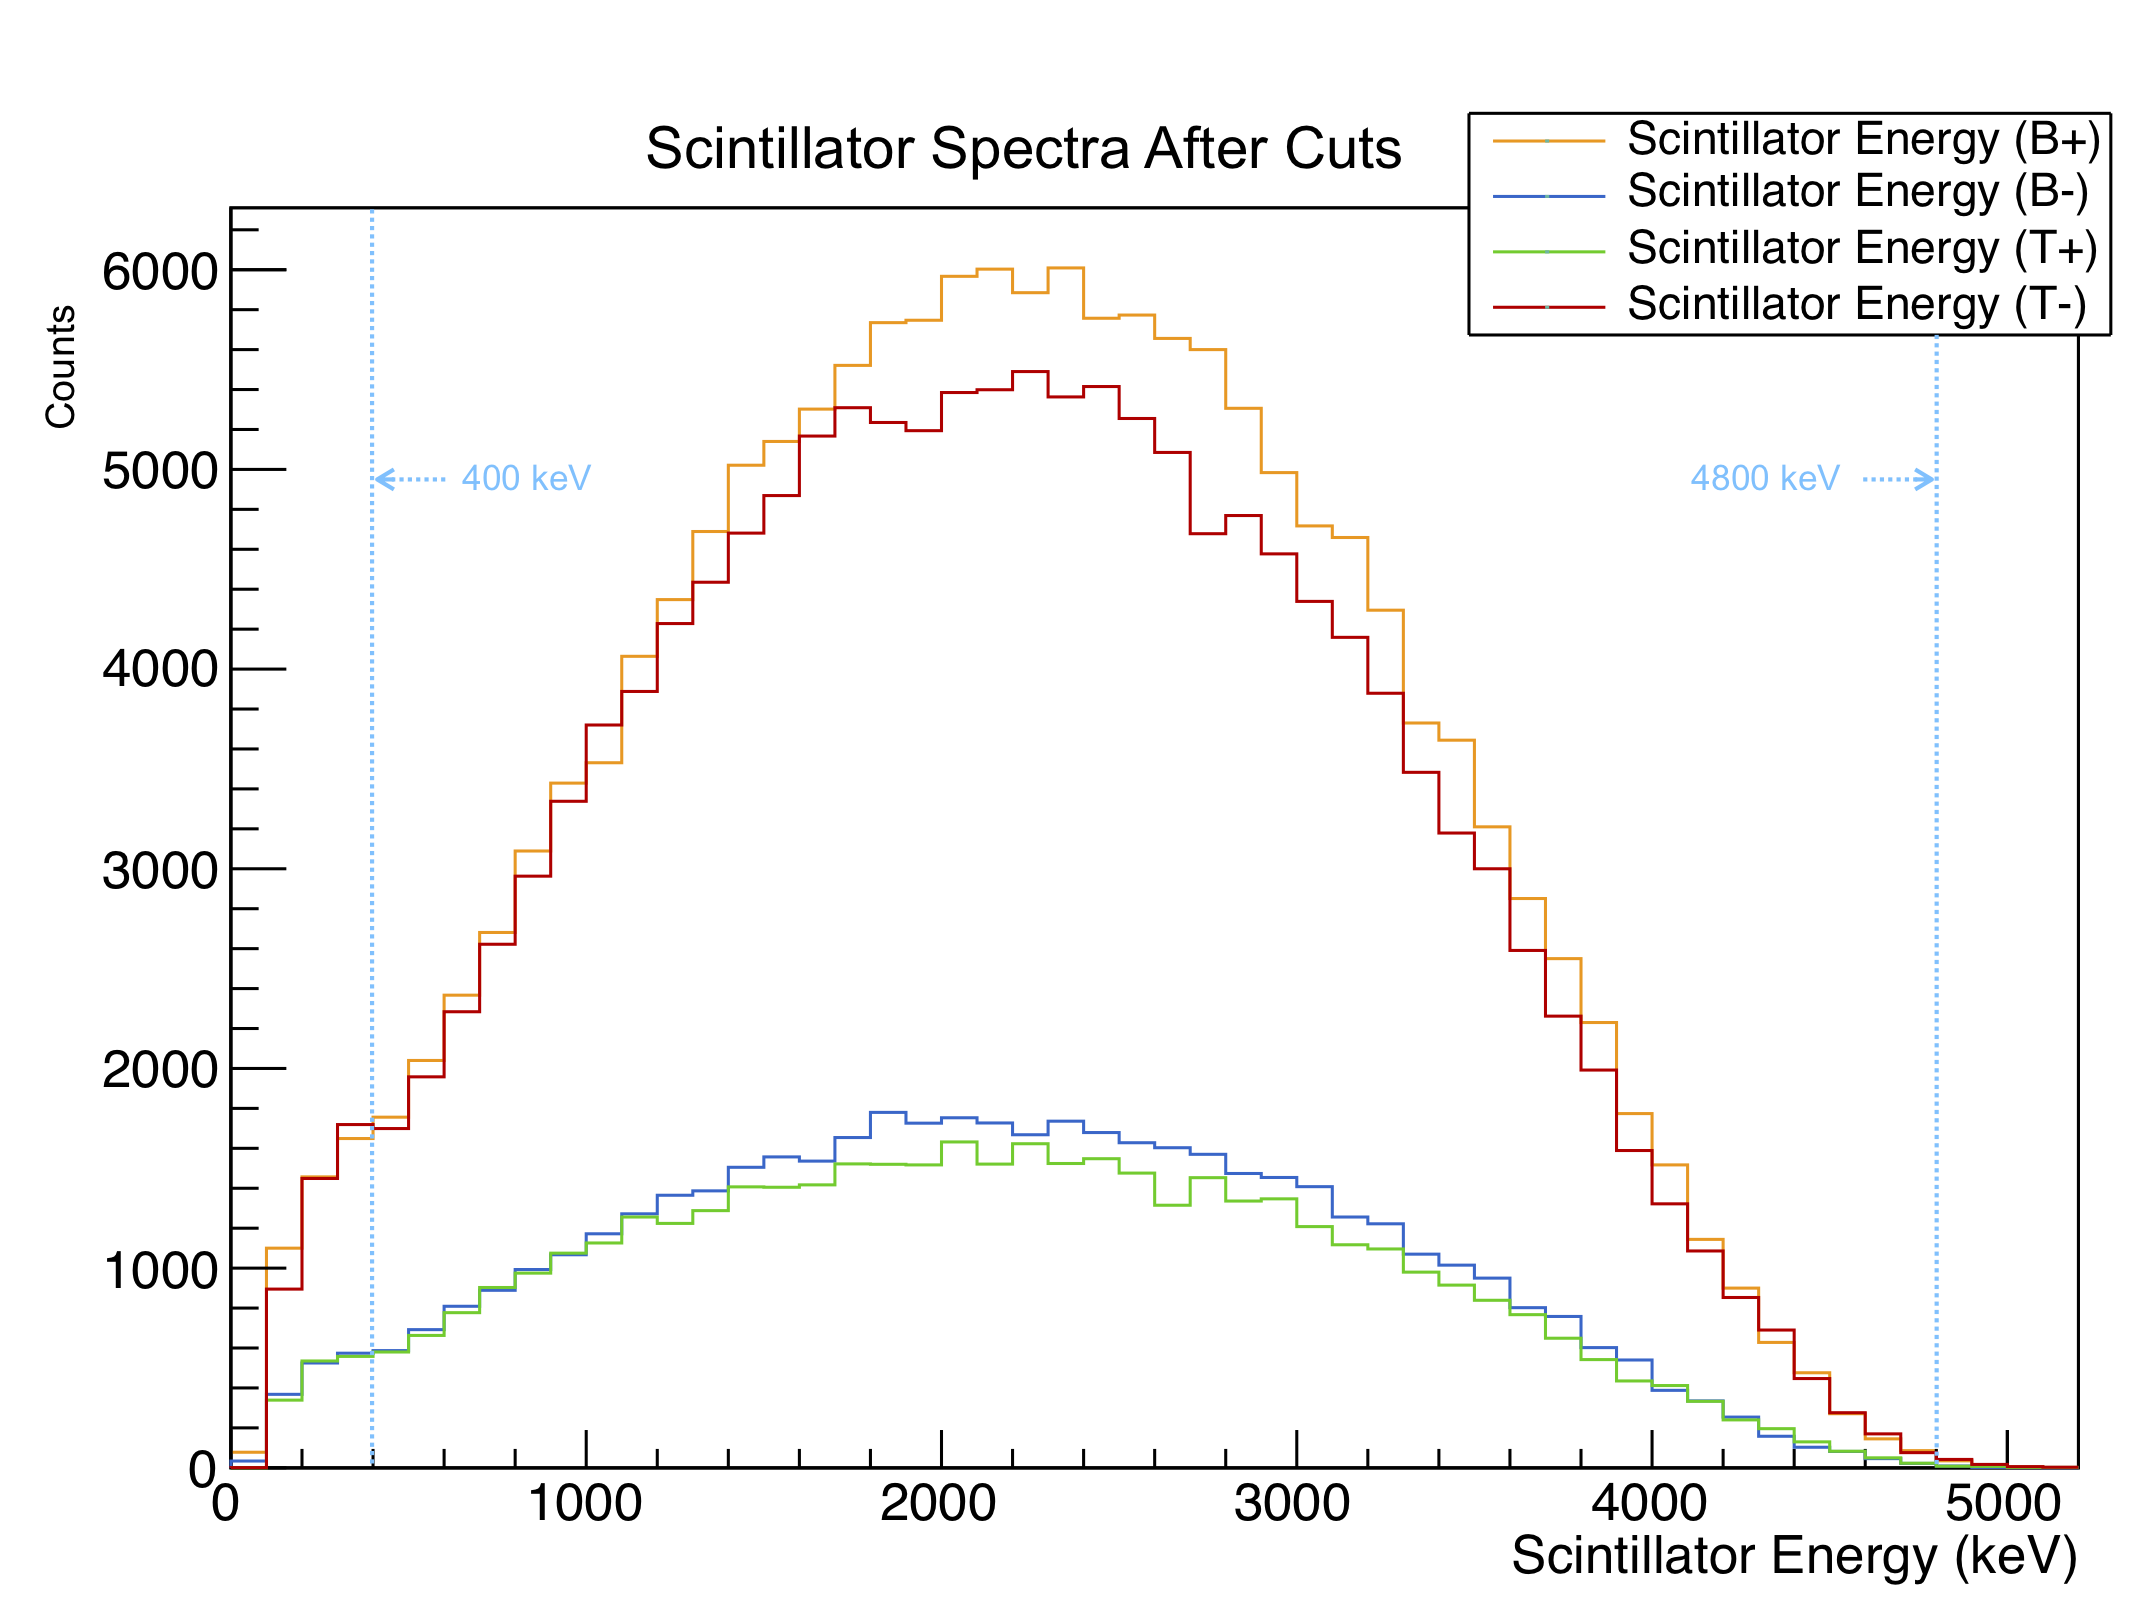
\includegraphics[width=.999\linewidth]
	{Figures/experimental_scintspectra_lin.png}
	\caption[Experimental Scintillator Spectra]{Experimental Scintillator Spectra, for both detectors in both polarization states.  These spectra are what remain after all cuts have been taken.  All runsets are included.}	
	\label{fig:scintspectra}
	\note[color=tag]{Experimental scint. spectra plot needs to be referenced in text.}
\end{figure}





%With the Data:  Make some more careful cuts to clean the data.  
%	%	\begin{itemize}
%%		\item \greycomment{Discard events without a ``good'' DSSD hit.  Eliminates vast majority of background 511s.  Necessitates having a definition of what a ``good'' DSSD hit is.  It's subtle enough that we'll want to leave some part of this definition of ``good'' to be varied as a systematic effect.  Notably, we consider energy agreement for each hit pixel, individual strip SNR, and overall DSSD energy threshold.  Also, hit radius w.r.t. center of detector.  This is a lot of stuff, all implemented by Ben -- and it needs to be done fairly early on in data processing in order to keep processing times for everything else manageable.  }
%		\item Discard events where SOE-Beta TOF falls outside a certain range.  Necessitates picking a ``good'' range.  The precise definition of ``good'' is varied as a systematic.  
%		\item \greycomment{Could have implemented an eMCP hit *position* requirement, but that kills too many stats.  It's like a factor of two.}
%	%	\end{itemize}
%\end{itemize}






